\documentclass[10pt]{article}

% amsmath package, useful for mathematical formulas
\usepackage{amsmath}
% amssymb package, useful for mathematical symbols
\usepackage{amssymb}

% graphicx package, useful for including eps and pdf graphics
% include graphics with the command \includegraphics
\usepackage{graphicx}

% cite package, to clean up citations in the main text. Do not remove.
\usepackage{cite}

\usepackage{color} 

% Use doublespacing - comment out for single spacing
\usepackage{setspace} 
\doublespacing

% Text layout
\topmargin 0.0cm
\oddsidemargin 0.5cm
\evensidemargin 0.5cm
\textwidth 16cm 
\textheight 21cm

% Bold the 'Figure #' in the caption and separate it with a period
% Captions will be left justified
\usepackage[labelfont=bf,labelsep=period,justification=raggedright]{caption}

% Use the PLoS provided bibtex style
\bibliographystyle{plos2009}

% Remove brackets from numbering in List of References
\makeatletter
\renewcommand{\@biblabel}[1]{\quad#1.}
\makeatother


% Leave date blank
\date{}

\pagestyle{myheadings}
%% ** EDIT HERE **


%% ** EDIT HERE **
%% PLEASE INCLUDE ALL MACROS BELOW

\usepackage{multirow}
\renewcommand{\arraystretch}{1.1}

% figure files reside in the figures/ directory
\graphicspath{
{figures/}
}

\usepackage{color}
\usepackage[usenames,dvipsnames,table]{xcolor}
\usepackage{ulem}

\definecolor{dkred}{rgb}{0.75,0,0}
\definecolor{dkgreen}{rgb}{0,0.5,0}
\definecolor{dkblue}{rgb}{0,0,0.75}
\definecolor{dkpurple}{rgb}{.375,0,.375}
\definecolor{gray}{rgb}{0.5,0.5,0.5}

\newcommand{\removed}[1]{{\color{dkred}\sout{#1}}}
\newcommand{\drew}[1]{{\color{dkgreen}#1}}
\newcommand{\fred}[1]{{\color{dkblue}#1}}
\newcommand{\steph}[1]{{\color{dkpurple}#1}}

%% END MACROS SECTION

\begin{document}

% Title must be 150 characters or less
\begin{flushleft}
{\Large
\textbf{Chemokines versus viral replication: a spatial of model of lymphocyte search in the influenza infected lung}
}
% Insert Author names, affiliations and corresponding author email.
\\
Drew Levin$^{1,\ast}$, 
Stephanie Forrest$^{1}$, 
Soumya Banerjee$^{1}$,
Candice Clay$^{2}$, 
Judy Cannon$^{3}$,
Melanie Moses$^{1}$, 
Frederick Koster$^{1,2}$
\\
\bf{1} Department of Computer Science, University of New Mexico, Albuquerque, NM, USA
\\
\bf{2} Lovelace Respiratory Research Institute, Albuquerque, NM, USA
\\
\bf{3} Department of Molecular Genetics \& Microbiology Department of Pathology, University of New Mexico Health Sciences Center, Albuquerque, NM, USA
\\
$\ast$ E-mail: Corresponding drew@cs.unm.edu
\end{flushleft}



% Please keep the abstract between 250 and 300 words
\section*{Abstract}

Emerging strains of influenza, such as avian H5N1 and 2009 pandemic H1N1, are more virulent than seasonal H1N1 influenza, yet the underlying mechanisms for these differences are not well understood.  Viral clearance depends in part on the ability of T cells to locate the infection in time to prevent uncontrolled spread of the virus.  We use an agent-based spatial model to quantify how efficiently T cells locate and control different strains of influenza in the lung.  We calibrate the model using viral and chemokine secretion rates measured \textit{in vitro} for avian H5N1, seasonal H1N1, and 2009 pandemic H1N1 influenza, together with values taken from literature.  The spatial model reveals challenges for T cell recruitment not apparent in standard differential equation models.  The model shows that virus kinetics largely determine the course of the infection, while T cell chemokine parameters have less effect.

%Further analysis of the model identifies the viral parameters as most significant and suggests possible mitigation strategies.

% ---- 300 word abstract

% Emerging strains of influenza, such as avian H5N1 and 2009 pandemic H1N1, are more virulent than seasonal H1N1 influenza, yet the underlying mechanisms for these differences are not well understood.  Subtle differences in how a given strain interacts with the immune system are likely a key factor in determining virulence.  One aspect of the interaction is the ability of T cells to locate the foci of the infection in time to prevent uncontrolled expansion.  Here, we focus on T cell navigating from the lymph nodes through the vascular system to the infection, using an agent-based spatial model to investigate how different strains of influenza influence the efficiency of this process.

%We calibrate the model using viral and chemokine secretion rates measured \textit{in vitro} for avian H5N1, seasonal H1N1, and 2009 pandemic H1N1 influenza, together with values taken from literature when available.  The spatial nature of the model reveals unique challenges for T cell recruitment that are not apparent in standard differential equation models. As plaques expand in size, the ratio of infected cells to dead cells decreases, making it difficult for T cells to encounter infected cells efficiently.  Further, differences in diffusion rates between chemokines and virions can misdirect T cells to areas that no longer contain infected epithelial cells.  Sensitivity analysis of the model identifies the viral parameters as the most significant factor in determining the course of the resulting infection.  Finally, we use the model parameters to determine an upper bound on T cell search time in the model.

% ---- end 300 word abstract

% To determine local chemokine production, avian H5N1, seasonal H1N1, and 2009 H1N1 pandemic influenza strains were used \textit{in vitro} to induce the secretion of CXCL10 (IP-10) and CCL5 (RANTES) in human bronchial epithelial cells.  These data were fit to a differential equation model in order estimate viral and chemokine production rates. 

% Infected cells can become isolated in expanding plaques, impeding T cell search, even though the T cells could directionally migrate to low levels of chemokine.  This spatially explicit model describes efficient T cell recruitment to small infected foci in the lung, but as foci become large T cell search becomes inefficient, thus emphasizing the importance of enhanced control early in infection.  A key limitation imposed on T cells is illustrated by their failure to clear the pandemic H1N1 virus after day 6, when T cells became inefficient in finding infected cells in large foci.    Thus, we conclude that viral dynamics, rather than chemokine dynamics, dominate the efficiency of T cell recruitment in determining whether the influenza infection is controlled.


% Please keep the Author Summary between 150 and 200 words
% Use first person. PLoS ONE authors please skip this step. 
% Author Summary not valid for PLoS ONE submissions.   
% \section*{Author Summary}

\section*{Keywords}

Agent-Based Model, Systems Biology, Immunology, Computational Biology, Virology


\section*{Introduction}

Influenza has worldwide epidemic potential with 5 million infections annually and half a million deaths \cite{Who2009}.  Emerging strains of influenza, such as 2003 H5N1 avian and 2009 H1N1 pandemic, are more pathogenic than seasonal strains, yet the the mechanisms that control this variability are not well understood.  Pathogenicity is a function of the virus and its interaction with the host immune response.

{\color{dkblue}Identifying the critical components of this complex process is key to understanding viral pathogenicity and designing therapeutic interventions.  However, determining the relative contribution of these myriad experimental components is challenging.  In this study, human epithelial cells were infected with Avian, seasonal, and pandemic influenza \textit{in vitro} and were measured for virus and various cytokine concentrations over the course of 48 hours.  The cytokine profile revealed that the only difference between influenza strains in epithelial cells is in the production of chemokines CXCL10 (IP-10) and CCL5 (RANTES).  Normally chemokines attract T cells to infection sites, and because \textit{in vivo} cell movement in lung tissue cannot be observed directly, we developed a model to examine this effect.}

%We address this challenge with computational modeling, which gives us the advantage of studying relative contributions of different aspects of the host immune response and accounts for strain-specific viral dynamics in the model.

Rather than developing a comprehensive immune system model, we focus on the role of chemokines in directing antigen-specific CD8 T cells from the lymph node to the focus of infection (FOI) in the human lung.  We assume that chemotactic gradients play an important role in guiding T cells to the FOI and that T cells resist extravasation and recirculate in the absence of inflammatory signals.  Chemotactic proteins are known to enhance T cell recruitment in both acute infections and chronic inflammatory diseases \cite{Bromley2008, Medoff2005, Castellino2006 ,Gunn1998, Okada2005}, where recruited T cells mediate either protection or immunopathology.  Infected epithelial cells secrete chemokines \cite{Chan2005}, and contact with CD8 T cells also triggers secretion \cite{Zhao2000}. Activated CD8 T effector cells upregulate chemotactic protein receptors, particularly CXCR3 and CCR5 \cite{Hoji2005, Groom2011a}, responding to their primary ligands IP-10 and RANTES respectively.  Previous work showed that efficient recruitment of T cells to the FOI is crucial for the eventual clearance of the virus \cite{Cerwenka1999, Kim2011}.  We extend this work to examine how the unique properties of the different strains of influenza may affect this process.

Because the recruitment of T cells through chemotaxis is a spatial process, we present a spatial agent-based model (ABM) of the secondary immune response to an influenza infection in the lung.  Previous models have shed light on the details of the primary and secondary immune response, some by applying ordinary differential equation (ODE) models to empirical data \cite{Miao2010, Saenz2010, Handel2008, Lee2009, Murillo2013}, and some by using spatial models to examine the interactions between dendritic cells and T cells in the lymph node \cite{Beltman2007, Zheng2008, Vroomans2012, Textor2014}.  We parameterize our model with \textit{in vitro} generated measurements of viral expansion dynamics as well as published data of host immune responses to flu infection.  The model was used to determine the pathogenic potential of the three individual flu strains: seasonal H1N1 (sH1N1), Avian H5N1 (aH5N1), and pandemic H1N1 (pH1N1).  These three strains were selected for their differences in \textit{in vitro} replication rates \cite{Mitchell2011} as well as differences in \textit{in vivo} severity of human and animal pneumonia and mortality.  The model describes the dynamic, spatially explicit evolution of viral infections in the context of the developing CD8 T cell response.  Sensitivity analysis shows most chosen model parameters have a limited effect on the qualitative results.   Those that have a strong effect are candidates for explaining the dramatic observed differences in pathogenicity among these different flu strains.

% The model design allows us to compare between influenza strains how the T cell response is affected by the viral and immune system characteristics.  The results show that efficient T cell search is crucial to viral clearance in the model and that the search process is dependent on more than just the replication rate of the virus, including the spatial landscape of the chemokine gradient and the location and density of virus-secreting cells.

{\color{dkblue}The main contributions of this paper are as follows.  First, \textit{in vitro} influenza infection of human epithelial cells stimulated production of chemokines IP-10 and RANTES, suggesting that these two chemokines play a direct role in recruiting T cells to the focus of infection.  Second, the spatial nature of the model allows us to identify physical constraints on T cells' ability to clear the rapidly replicating pH1N1 infection.  Because T cells in the model use the chemokine gradient to locate the FOI, they tend to cluster in areas of high chemokine concentration.  The model suggests that the chemokine response of the host cells may actually hinder T cells' ability to find and clear infected cells in the presence of the rapidly replicating pandemic strain.  Finally, the sensitivity analysis shows the isolated effects of each parameter in the model.  Based on this analysis, each parameter was classified as sensitive or not.  We find that most parameters can be individually varied across a broad range of values without strong effect on predicted outcomes.  Further, the parameter classification is consistent across each broad parameter type. Specifically, chemokine-related parameters are stable within biologically plausible ranges.  In contrast, parameters related to viral kinetics have a strong effect on model results.  We conclude that influenza infection dynamics are dominated by the replication properties of the virus and spatial properties of the infection, confirming that the higher replication rate of 2009 pH1N1 influenza obscured contributions of the chemotactic signals, leading to uncontrolled infection \textit{in silico}.}

% fred used 'obscured' instead of overwhelmed

% The model predicts the control and clearance of the aH5N1 and sH1N1 strains and predicts a runaway infection for the pH1N1 strain.  These results are consistent with the previously reported replication rates of the three strains of influenza.  

%  Infected cells secrete chemokine molecules which then diffuse across the infected region.  This process creates isolated regions, or local maxima, of high chemokine concentrations.  

% While the local maxima do move and flatten, their speed is limited by their diffusion and decay rates.  


% You may title this section "Methods" or "Models". 
% "Models" is not a valid title for PLoS ONE authors. However, PLoS ONE
% authors may use "Analysis" 
\section*{Materials and Methods}

% We are interested in how the interaction between the virus and the host's secondary immune response affects the virulence of the infection.  Because these interactions are difficult and expensive to observe \textit{in vivo}, we create a model \textit{in silico} to represent the system in question.  Because we are interested in individual interactions between the virus and the immune response, as well as the spatial nature of the spreading infection and the subsequent T cell search, we eschew traditional differential equation models \cite{Beauchemin2006a, Bauer2009} in favor of a spatial agent-based model (ABM).  

% Our modeling methodology follows three steps.  First, we define the system we are going to model.  Second, we build the model with this definition in mind.  Finally, we parameterize the model using empirical data, values from literature, and computational techniques.

\subsection*{Model Definition}

%Our model examines the secondary immune response to an influenza infection in a human lung.  Specifically, we are interested in how antigen activated T cells efficiently navigate from the lymph node, through vascular system, and into the lung at the site of infection.  

The model focuses on activated CD8 T cells migrating through the vascular and lymph networks, including their movement over tissue after extravasation (Fig.~\ref{fig:systemchart}).  {\color{dkblue}While the volume of the lung consists of spherical alveoli, the spread of influenza throughout the lung occurs through the interconnected bronchiole-alveoli complex, which can be viewed as a connected monolayer.  Thus, we represent the lung as a two-dimensional sheet of healthy epithelial cells (S1.3).}   Because we assume activated T cells descend at random into branches of the vascular network, T cells in the model are introduced uniformly at random across the modeled lung surface.  If cytokine signal is detected on the local endothelium the T cell remains in tissue and follows the chemotactic gradient to the FOI.  T cells that do not encounter cytokine recirculate to the lymph node where they reenter the bronchial vascular network.  Once inside the endothelium, T cells follow the chemokine gradient to localized areas of maximum chemokine concentration.  When a T cell contacts an infected epithelial cell it induces apoptosis (S1.4).  Otherwise, infected cells continue to secrete virus for a fixed time and then die.

The model is initialized with a single infected cell.  After the incubation period, the infected cell begins secreting virus and chemokine at rates determined by the virus strain and chemokine type (S2.1 and Table \ref{tab:strains}).  Virus from expressing cells diffuses locally, infecting neighboring cells. Chemokine diffuses from secreting cells, creating a spreading region of stimulation around the FOI. After five simulated days, representing lymph node stimulation and T cell proliferation, activated T cells exit the lymph node at a constant rate and travel through the vasculature to the tissue as described above.  These cell and molecular interactions and state transitions are depicted in Figure~\ref{fig:systemchart}.

\subsection*{Model Implementation}

The model is implemented using the CyCells software \cite{Warrender2006} (\texttt{https://github.com/drewlevin/cycells}), a modeling platform for two- or three-dimensional agent-based simulations of the immune response (S1.1).  Due to computational constrains our model is scaled to the size of a mouse lung (approximately 100$cm^2$), a well-established practice in spatially explicit influenza models \cite{Miller2003, Allan2006, Ingulli2009}.  Parameters affected by this choice include the T cell production rate, T cell circulation time, and the total size of the lung (Table \ref{tab:parameters}).

Parameters that are independent of the chosen influenza strain are shown in Table \ref{tab:parameters}.  Strain-specific values are shown in Table \ref{tab:strains}.  Further details regarding the model definition are included in S1.2.

In the model, epithelial cells are stationary and are described by one of five sequential states: \texttt{healthy}, \texttt{virus-incubating}, \texttt{virus-expressing}, \texttt{apoptotic}, and \texttt{dead} \cite{bachem1996simulated, Beauchemin2005, Mitchell2011}. \texttt{Healthy} cells remain unchanged unless infected by virus. Once infected, the cell transitions from \texttt{incubating} to \texttt{expressing} after a 10 hour incubation delay. \texttt{Expressing} cells secrete virus and chemokine for a fixed 16.7 hours and then die. \texttt{Expressing} cells initiate apoptosis sooner if they are contacted by activated T cells. \texttt{Apoptoic} cells continue to secrete virus and chemokine and then die after one hour. \texttt{Dead} cells take up space and do not regenerate over the course of an infection.  Cell regrowth is not implemented as the rate of regrowth is unknown. 

T cells are described by two states: \texttt{circulating} and \texttt{chemotaxing}.    T cells emerge from the lymph node at five days post infection (p.i.) at a rate of 1,257 cells per hour. T cell travel time from the lymph node to a random location on the lung's surface is six seconds.  If chemokine is not encountered, the circulating T cell returns to a new location in the lung after another six seconds.  If a circulating cell encounters chemokine, it changes state to \texttt{chemotaxing} and follows the chemotactic gradient to the FOI. Circulating T cells decay exponentially with an average lifespan of three days.  Chemotaxing T cells follow the gradient through the two-dimensional lung endothelium, inducing apoptosis when they encounter expressing epithelial cells. Chemotaxing T cells decay exponentially with an average lifespan of two hours.

In addition to T cells, the model contains two types of particles: virus and chemokine. Both are produced at constant rates by expressing epithelial cells.  Virus diffuses through the lung tissue, infecting healthy cells at a rate proportional to the virus concentration at the location of the cell. Chemokine diffuses across the tissue but has no direct effect beyond recruiting T cells. Both particle types decay exponentially.  IgM is modeled by increasing the viral decay rate by a factor of ten after the fourth day.


\subsection*{Model Parameters}

Model parameters are listed in Tables \ref{tab:strains} and \ref{tab:parameters}. These values were taken from the literature when available.  Other parameters were determined experimentally, and some parameters were estimated using biologically plausible ranges.  All estimated parameters were studied in a sensitivity analysis to test their impact on model behavior. 

Because we are interested in the interplay between the virus and the induced immune response, we infected human epithelial cells with the three different strains of influenza \textit{in vitro} and measured the resulting cytokine and chemokine responses.  We extended a previously published differential equation model \cite{Mitchell2011} to obtain values for per-cell chemokine production rates (S2.1).  T cell production rates were derived from measured replication rates \textit{in vitro} \cite{Miao2010} using another differential equation model (S2.2). T cell production is assumed to be constant after day 5 \cite{MartIn-Fontecha2003}.  

\subsection*{Materials}

In an effort to obtain per-cell chemokine and cytokine production rates, human epithelial cells were infected with influenza \textit{in vitro}.  Epithelial cell culture and supernatant collection was performed as described in \cite{Mitchell2011}.  Briefly, undifferentiated human tracheal epithelial cells (University of Miami) were cultured for 4 weeks to achieve fully differentiated confluent monolayers on collagen-coated transwell inserts, or commercial differentiated human bronchial epithelial cells (EpiAirway Tissue, MatTek Corp., Ashland, MA) used immediately upon receipt, were infected at an MOI of 0.01 with either seasonal H1N1 virus A/New Caledonia/20/99 (sH1N1), the 2009 H1N1 pandemic strain A/California/04/09 (pH1N1), or avian H5N1 virus A/Hong Kong/483/97 (aH5N1) derived from a fatal human infection.  Basal media was collected from previously undisturbed triplicate or quadruplicate wells at 0, 6, 10, 12, 16, 20, 24, 30, 36, 42, 48, and 72 hours after infection, and stored at -80C until assay.  Subsequently, apical fluid for virus secretion was collected before and after treatment of the monolayer with protease (Pronase, Sigma) to optimize the collection of infectious virus \cite{Mitchell2011}.  Quantitative viral culture was performed by standard plaque assay.  Quantitative chemokine levels were performed in 30 $\mu$L aliquots for a panel of chemokines (IL-8, MCP-1, MIP-1$\alpha$, MIP-1$\beta$, RANTES, IP-10, eotaxin) and cytokines (interferon-gamma, IL-1$\alpha$, IL-1$\beta$, IL-1RA, IL-2, IL-3, IL-4, IL-6, IL-10, IL-12p40, IL-15, IL-17, TNF$\alpha$) (Luminex Assay®, Luminex Corp.) and reported as ng/mL basal media sampled from a total volume of 4 mL.  Only IP-10, RANTES, and TNF$\alpha$ showed increases in production (Table S1).  TNF activity is not incorporated in the model.  Data for other chemokines and cytokines is not shown.



\section*{Results}

\subsection*{Model Results}

Because the CyCells model is stochastic, we conducted 50 runs of the model for each of the three strains, each run initialized with a unique random seed (Fig.~\ref{fig:variance}).  For the avian and seasonal strains, all model runs cleared the virus by day 10.  Conversely, each simulation of the 2009 pandemic influenza led to runaway infection.

% We estimated variance across the runs using the $R^2$ statistic, $\pm$ one standard deviation: 0.957 $\pm$ 0.150 (avian), 0.992 $\pm$ 0.013 (seasonal), and 0.998 $\pm$ .002 (pandemic).  The $R^2$ was computed with respect to the mean number of infected cells at each simluated time point across all 50 runs. Consistent with earlier results \cite{Mitchell2011}, the time course of the infection varies significantly across the three strains (Fig.~\ref{fig:variance}).

We estimated variance across runs by calculating the standard deviation at each time point.  For aH5N1, the maximum standard deviation was 37, which occurred at day 5.05 where the mean value was 259.  For sH1N1, the maximum standard deviation was 242, which occurred at day 4.93 where the mean value was 2,607.  For pH1N1, the maximum standard deviation was 230, which occurred at day 5.07 where the mean value was 7,018.

In all studied strains, virus expansion declines at four days p.i. (Fig.~\ref{fig:variance}), due to IgM appearance.  Subsequently, the simulated CD8 T cell response causes the number of infected cells to decline quickly after day five p.i.  aH5N1 is cleared completely, sH1N1 is cleared more slowly, and at day six p.i., pH1N1 replication dominates the IgM and T cell response.  These results agree with previously reported \textit{in vivo} differences among the three different strains \cite{Mitchell2011}.

% Interestingly, the attenuation of the type I interferon response by H5N1 viruses is not associated with attenuation of chemokine secretion in our results and in others \cite{Zeng2007}.  

% The rapid production of the pH1N1 virus prevents the immune response from containing the infection (Fig.~\ref{fig:variance}C).  Because pH1N1 replicates more rapidly, the number of infected cells outstrips the ability of the T cells to find them.   Spatial effects reveal the reasons for this in simulation images and video (Fig.~\ref{fig:cycells}, Video S4). 

\subsection*{Spatial Effects}

% Free virus particles diffuse from virus secreting cells and infect healthy cells.  Chemokine produced by infected cells attracts T cells to the infected cells.

Plaque growth in the model is illustrated in Figure \ref{fig:cycells}.  Because the virus particles are an order of magnitude larger than the chemokine molecules, they diffuse more slowly, according to the Stokes-Einstein equation.  However, chemokine molecules decay more quickly than the virus (Table~\ref{tab:parameters}).  In the model these countervailing forces produce similar spatio-temporal profiles for the two particle types (Fig.~\ref{fig:cycells}). Before day 4 the plaque is dominated by active (incubating and secreting) cells, with a small percentage of dead cells (Panel A). Over time, cells in the plaque's interior die, and active cells comprise a decreasing proportion of the plaque. T cells arrive at day 5 and begin killing the virus-secreting cells (Panel B). By day 6 many expressing cells have been eliminated and the plaque is dominated by dead cells (Panel C).  Although not visible in the figure, plaque size and T cell number changes continuously for all strains and is demonstrated for seasonal H1N1 virus (Videos S1-S3).

In the aH5N1 infection, the plaque is densely populated with infected cells, allowing T cells to find secreting cells easily and clear the infection (Figs.~\ref{fig:plaquesize}A).  However, secreting cells were not cleared in either the sH1N1 or pH1N1 simulations (Fig.~\ref{fig:variance}).  In these runs, secreting cells accounted for at most 10\% of the active cell population and less than 1\% of the total plaque at 6 days p.i. (Fig.~\ref{fig:plaquesize}).  T cells continue to accumulate, but they arrive at a slower rate than the rate at which new cells become infected.  Further, the newly arriving T cells are less efficient because the epithelial cells are more sparsely distributed in the plaque.

Finally, the spatial nature of our model reveals that regions of concentrated chemokine diffuse more slowly than the ever-expanding infected cell and virus locations, thus misdirecting the chemotaxing T cells.  It takes time for infected cells to begin producing chemokine, while the preexisting pockets of high chemokine density are slow to decay.  Thus, T cells whose movements respond to the spatial layout of the chemokine gradient can become trapped, failing to locate new regions of infected cells in the growing plaque.  This effect is most pronounced in the pH1N1 strain, where the plaque expands more quickly than the chemokine can diffuse.

% Taken together, the delayed response and low proportion of virus secreting cells contribute strongly to the failure of T cells clearing the infection.  Furthermore, increasing chemokine production fails to guide T cells to the actively secreting epithelial cells in the runaway pH1N1 infection (Fig. S5), suggesting that the effect of high viral production rates dominate increased chemokine production rates.


\subsection*{Sensitivity Analysis}

% One advantage of computational modeling is the ability to manipulate the model in ways not available in the real system.  Here, we have taken advantage of our model by adjusting each parameter in question while holding the rest constant.  This sensitivity analysis allows us to make two main observations.  First, we can directly examine how each component of the model affects the final behavior of the model.  Second, we can determine which model parameters are sensitive (those that affect the model's behavior) and which are stable (those which do not affect the model's behavior).[TODO move somewhere or delete]

We conducted a sensitivity analysis of sixteen model parameters to identify those that are most important for determining model outcomes.  We studied all but five of the parameters listed in Tables~\ref{tab:strains} and \ref{tab:parameters}, excluding T cell radius, T cell sensitivity to chemokine, T cell onset time, IgM onset time, and the viral production rate.  T cell radius is known \cite{abbas2011cellular} and does not factor strongly into the spatial model's implementation.  T cell sensitivity was set arbitrarily to mimic a realistic threshold of response to cytokine (S2.3).  The two onset parameters are known \cite{Diamond2003}.  Viral production is an independent variable, as discussed above, and determined by each of the three strains \cite{Mitchell2011}.

Each of the remaining sixteen parameters was varied independently (over multiple orders of magnitude when appropriate) for each viral strain, and the model was rerun once for each parameter setting.  Results were compared for the quantitative size of the peak infection and the number of uncleared infected cells at day 10 p.i.  Based on these runs, we classified each parameter for each strain as follows (Table~\ref{tab:sensitivity}): \textit{stable} parameters are those that do not affect the model behavior over any of the different values tested; \textit{bounded stable} parameters are stable throughout a reasonable range of values but model behavior diverges at some threshold; \textit{peak change} parameters affect the peak size of the infection, but do not change the ultimate number of infected cells at the end of the run; and \textit{sensitive} parameters affect the behavior of the model whenever they are changed.

Table \ref{tab:sensitivity} shows that four parameters are sensitive: viral response to IgM, infectivity, viral decay rate, and viral diffusion.  In addition, Figure \ref{fig:variance} shows that viral production rate is a sensitive parameter due to the difference between the three panels.  The four parameters (infectivity, viral decay rate, viral diffusion rate, and viral production rate) are specific viral characteristics.  Further, viral response to IgM, as coded in the model, directly affects viral decay rate and can be included in this group.  None of the remaining T cell parameters or the chemokine parameters have a strong effect on the model's prediction of control or lack of control of viral replication.  This result supports the hypothesis that virus dynamics dominate the course of an influenza infection.  


\subsection*{Window of Control}

Our sensitivity analysis suggests that viral parameters are the most sensitive and have the largest effect on the the course of the infection (Table~\ref{tab:sensitivity}).  We asked whether T cells could play a role by assessing multiple factors that control the overall T cell response.  Here, we define the window of control as the maximum time virus-secreting cells may produce virus while still allowing the infection to be cleared.  This window can be defined as the combination of the the time of T cell arrival at a virus-secreting cell ($T_{arr}$), the time it takes for the T cell to induce apoptosis ($T_{kill}$) and the time for the infected cell to apoptose ($T_{apop}$).

An epithelial cell infected with pH1N1 produces new virus at the rate of 5.08e-3 PFU/s (Table~\ref{tab:strains}).  Using the parameters from Table \ref{tab:parameters}, T cell-induced apoptosis occurs within 10 minutes of T cell arrival, viral secretion continues for one hour after apoptosis is initiated, and under these circumstances the cell produces 21 new viral particles that can infect new cells.  In contrast, with the sH1N1 strain, a single infected cell produces 1.6 viral particles in the 70 minute window, and for the aH5N1 strain this number is 0.2.  % Thus, viral clearance depends on the interaction of the rate of apoptosis, viral decay, viral production, and the viral infection probability.  

Even if T cell arrival and apoptosis time were instantaneous, a cell would still secrete virus for 10 minutes ($T_{kill}$), producing 3 new virions in the case of pH1N1.  Only in the case where both $T_{kill}$ and $T_{apop}$ are simultaneously reduced can the pandemic infection be cleared.  We confirmed this effect in the model by first setting both relevant parameters (apoptosis time and T cell kill time) to zero, and as expected all three strains were cleared (Fig.~\ref{fig:instantkill}).  We now ask how much T cell delay the model can tolerate and still clear a given viral strain.  To answer this, we formulate the basic equations of the model in terms of $R_0$, the viral replication rate, and solve for the case where $R_0 < 1$.

\begin{equation}
R_0 = p \times (T_{arr} + T_{kill} + T_{apop}) \times E
\end{equation}

\noindent where $p$ is the secretion rate of the virus and $E$ is viral effectiveness, i.e. the proportion of virus that infects cells.  Equation 1 assumes each free virus particle can infect no more than one healthy epithelial cell.

%%%
% Note that this equation calculates the number of virions that may be produced by an infected cell, but omits the number of cells that can subsequently be infected by the virus.  A quick calculation of a virion's expected life span in the presence of IgM (2.4 hours) combined with the expected time it takes to infect a healthy cell (2 hours), results in a value greater than one.  Given that virus is removed from the model when a cell becomes infected, each virus is limited to infecting one target cell, and thus this quantity does not affect the equation for $R_0$.

% $R_0$ can simplistically be defined as the viral production rate multiplied by the time of production.  Using this definition, the claculated $R_0$ of the sH1N1 virus is 1.6, suggesting growth, yet the actual infection is eventually cleared  by day 10 in our model.  This can be attributed to the spatial effects of the ever-expanding ring of infection.  
%%%

$p$, $T_{kill}$, and $T_{apop}$ are model parameters (Table \ref{tab:parameters}).  $E$ incorporates both spatial effects of viral diffusion and temporal effects of viral decay.  As the infected plaque expands, some secreted virus diffuses to cells that are already infected or dead (the existing plaque) and do not contribute to new infections.  This effect is minimal in the beginning when the edge of the plaque is small and tightly curved.  As the plaque expands, its radius grows and the edge approaches the limiting case of a straight line when 50\% of the virus could be expected to diffuse over healthy cells and 50\% over infected or dead cells.  In the presence of healthy cells, virions infect the cells at a rate of $0.5/h$ and decay at a rate of $0.42/h$ in the presence of IgM after day 4 p.i.  (Table \ref{tab:parameters}).  This suggests that 50\% of free virus contacts healthy cells and 54\% of that virus succeeds in infecting a healthy cell, implying that $E \approx 0.27$ (S2.6).  Solving for $T_{arr}$ where $R_0 < 1$ gives:

\begin{equation}
\lim_{t \to \infty} T_{arr} < \frac{1}{pE} - (T_{kill} + T_{apop})
\end{equation}

Using the model parameters, this equation suggests that $T_{arr} < 18h$ for aH5N1 and $T_{arr} < 93m$ for sH1N1.  pH1N1, however, cannot be cleared for any value of $T_{arr}$ in this scenario.  

The above calculation suggests a combined transition point for sH1N1 at 163 minutes ($R_0 = 1$ for $T_{arr}+T_{kill}+T_{apop}=163m$), which is consistent with the sensitivity analysis (Fig.~S4: Apoptosis Time: 90m - 120m) and suggests that the modeled $T_{arr}$ is between 33 and 63 minutes for sH1N1.  These data show that the balance between viral production and T cell response is a key factor in clearance of infection: pH1N1 can theoretically be cleared with instantaneous T cell responses, but in actuality viral production exceeds T cell response time and this leads to uncontrolled infection.


\section*{Discussion}

We used a spatial model to study how T cell search in the lung affects the host's ability to clear virus.  CD8 T cells conduct two `searches' in two different tissue environments, first to encounter antigen-loaded dendritic cells in the lymph node, and second to encounter local inflammatory signals in the infected lung.  Search problems in the lymph node have been simulated using live cell imaging data to provide reliable parameters of cell movement \cite{Vroomans2012}.  Our model focused on the second search, i.e. the process of recruiting activated CD8 effector cells to infected sites in the lung, which is not as well understood.  In contrast, the dense 3D lymph node volume, our model approximates a mouse lung as a 2D surface where the epithelial cell monolayer is 100 $cm^2$ (only the area containing the FOI is modeled explicitly).  T cells must somehow rapidly locate the infection, which at day 5 p.i. is approximately 0.5 $mm$ in diameter.  Our model revealed four main conclusions regarding chemokine aided T cell search in the lung.

First, confirming earlier results \cite{Mitchell2011}, the model consistently clears the aH5N1 strain by day 10 p.i., contains sH1N1 by day 10 p.i., and fails to clear the pH1N1 infection.  Second, the model revealed spatial constraints on T cell search when the infection spreads more quickly than the chemokine gradient can diffuse.  In these cases, T cells become trapped in areas of high chemokine concentration which lag behind the expanding infection.  High concentrations of chemokine also attract and trap arriving T cells, thus limiting the direct benefit of increasing numbers of T cells. Third, the sensitivity analysis tested the individual effects of each parameter on the model's behavior.  The analysis shows that virus kinetics largely determine the course of the infection, while T cell and chemokine parameters do not have a strong effect.  Finally, we examined the window of control which suggests that pandemic influenza could not be cleared even if apoptosis were instantaneous.  


% \subsection*{T Cell Recruitment}

% The naive T cell must encounter on average hundreds of irrelevant cells before it contacts the loaded DC, but the distance traveled is relatively short.  


% The initial localization and extravasation of T cells into the bronchial tissue may depend on a number of inflammatory signals, but viral antigen does not appear to induce recruitment into this tissue \cite{Topham2001}.   Moreover, the T cells leaving the lymph node are released into the very large systemic vascular `space' with no initial guiding signals.  Effector cells must localize to sites of viral replication \cite{Cerwenka1999}, but it is not clear whether cells passing through uninfected lung tissue leave through the pulmonary vein or exit the capillary bed and leave the lung through lymphatic channels. 

% In this paper, we assume T cells climb the chemokine gradient though ligand-receptor binding.  The consequences of chemotactic ligand-receptor interactions, however, are complex \cite{Groom2011a, Groom2011} and variable in the models studied.   For example, in the lymphochoriomeningitis virus model the CXCR3 receptor mediates T cell recruitment to infected brain and subsequent immunopathology \cite{Christensen2004, Christensen2006}, while the CCR5 mediates the opposite effect \cite{DeLemos2005}.  In contrast, in the West Nile virus model \cite{Klein2005} and the dengue model \cite{Hsieh2006}, deficiency of IP-10 reduced T cell recruitment to the brain resulting in higher viral burden and increased mortality.   In the herpesvirus model, IP-10 was critical in T cell recruitment and disease control in the HSV-2-infected brain \cite{Wuest2008, Thapa2008}.  In the parainfluenza virus model, CXCR3 receptor is critical in CD4+ T cell migration to the lung \cite{Kohlmeier2009}.  In the influenza A model, initial studies with chemokine receptor knock-out mice obtained mixed results with respect to changing the course of disease \cite{Dawson2000, Wareing2004}, concluding that redundancy in chemokine signals may confound interpretation.   The CXCR3 receptor mediated T cell localization and spared the increased mortality of CCR5 deficiency, but viral clearance was not altered \cite{Fadel2008}.  The CXCR3 receptor also mediates the balance between effector versus memory cell differentiation among recruited CD8 T cells in the lung \cite{Kohlmeier2011}.   

The \textit{in vivo} quantitative chemokine parameters in the infected lung are difficult to estimate.  There is clear evidence from multiple models that chemokines and chemokine receptors are required for effector T cell localization to infected tissues \cite{Christensen2004, Christensen2006, Dawson2000, DeLemos2005, Fadel2008, Gadhamsetty2014, Groom2011a, Groom2011, Hsieh2006, Klein2005, Kohlmeier2009, Kohlmeier2011, Thapa2008, Wareing2004, Wuest2008, Pawelek2012}. However, the actual effect of chemokines on effector T cells in tissues is still largely unknown.  Blood levels documented in virulent influenza infections \cite{DeJong2006} may not reflect lung tissue concentrations.  Dynamic chemokine concentrations secreted by bronchial epithelial cells \textit{in vitro} depend on infection intensity and cell maturation state \cite{Mitchell2011, Chan2010, Chan2005, Zeng2011} and may better approximate chemokine levels in tissue.  We have determined the level of chemokine released by infected bronchial epithelial cells (Table~\ref{tab:strains}) and used these as the best approximation for chemokine levels in tissues.  Our model did not incorporate the potential contributions from other chemokines such as CXCL8/IL-8 detected in bronchial cell cultures \cite{Matsukura1996, Arndt2002}, nor did the model account for chemokines secreted by immigrant macrophages \cite{Julkunen2000} and amplification of epithelial cell secretion by CD8 T cells \cite{Zhao2000}.  The sensitivity analysis classifies the chemokine secretion rate as stable, suggesting the total amount of chemokine is not a significant factor in determining viral clearance in our model.  

Although leukocytes exhibit directional behavior to chemokines \cite{LiJeon2002, McDonald2010}, CD8 T cells have not yet been shown to climb chemokine gradients.   While T cell chemotaxis may not be proven, previous work has shown severe limitations to viral clearance in the absence of this ability \cite{Banerjee2011}.  Our sensitivity analysis shows that reducing T cell velocity (and consequentially, the ability of T cells to climb gradients) hinders clearance of sH1N1 and pH1N1 strains.   These results are consistent with the hypothesis that T cells are guided by chemokine in the lung epithelium.

%Our model of T cell search is consistent with the literature and sheds light on T cell movement in the epithelium.

% Another key determinant in the efficiency of chemokine-directed T cell migration towards virus-secreting epithelial cells is the communication distance, defined by the threshold of sufficient chemokine signal required to induce directed motion of the cell up the chemical gradient \cite{Thelen2008}.  The diameter of this gradient generated by a single cell is a function of production rate, decay rate, protein diffusion and the sensitivity threshold.  For the threshold of 100 ng/mL and maximal levels of concentration in tissue of 10,000 ng/mL, we calculated the effective communication distance to be approximately 100 microns in our model by simulating a single chemokine producing cell and observing the radius of the resulting chemokine gradient.  This calculation is similar to the distance calculated for generic cytokines secreted by a suspended solitary cell \cite{Francis1997}.  




% \subsection*{Modeling Methodology}

% Previous works, including our own, have successfully used ODE population models to great effect.  Fitting the free paramters of ODE models to experimental data gives insights into the inner-workings of the system in question that are often not possible to obtain through direct observation and measurement.  Maio et al. uses ODEs to examine how the T cell response coupled with IgG and IgM affect influenza infection in mice \cite{Miao2010}.  Saenz et. al. examines the effect of the interferon response on influenza infection in equines \cite{Saenz2010}. Handel et. al. similarly uses ODE models to examine which immune responses dominate during the course of a influenza infection in mice \cite{Handel2008}.  Lee et. al. create a very comprehensive model of the adaptive immune response, including dendritic cells, CD4+ T cells, CD8+ T cells, and B cells \cite{Lee2009}.  Our previous work uses an ODE model influenza infection matched to \textit{in vitro} experimental data to estimate per-cell viral production rates for the three different strains of influenza discussed in this paper: aH5N1, sH1N1, and pH1N1 \cite{Mitchell2011}.

% These ODE models are effective approaches to estimate unmeasurable parameters of influenza infection and the subsequent immune response.  Unfortunately, ODE models are not adept at modeling spatial effects of the system in question.  Thus, other papers have successfully used spatial agent-based approaches to explore how spatial constraints affect the immune response to influenza infection.  Both Beltman et. al. \cite{Beltman2007} and Zheng et. al. \cite{Zheng2008} successfully use unique spatial models to examine how viral peptides are presented to unactivated T cells in the lymph node. 

% [MOVED UP] Here, we use spatial agent-based model (ABM) to examine the dynamics of how T cells locate and eradicate infected cells in the lung after they are activated in the lymph node.  Our use of an ABM has certain advantages over a spatially homogeneous differential equation model.  An ODE model assumes that any virus particle is capable of infecting any healthy cell.  Figure \ref{fig:cycells} shows that this is clearly not the case for viral adhesion and entry.  In fact, most free virus exists on top of infected cells that are no longer candidates for viral binding and fusion.  ODE models account for this discrepancy by lowering rates of infection by a constant amount, but this assumes that the proportion of unsuitable virions will always be the same.  This is limiting as can be seen in Figure~\ref{fig:cycells} where the early infection has a higher proportion of virus overlapping healthy cells.  Furthermore, explicitly modeling T cell chemotaxis reveals unique challenges to viral clearance brought about by infections that spread more rapidly than the chemokine gradient can decay and diffuse.

% A drawback of an agent-based model is the increased computational complexity when compared to a population model.  Rather than representing the agents as population totals, our model represents each one explicitly.  To account for this, our model necessarily makes a number of simplifications to and deletions of elements in the innate and adaptive system, including antigen presentation, clonal expansion, antibody affinity maturation, and other non-T cell involvement. While these parameters remain to be tested in other models, our current model allow us to build a tractable model of the aspects of the immune response necessary to explore specific aspects of virus and immune system interactions.  

% Finally, while our model is not meant to be biologically correct in the sense it does not attempt to replicate the entire immune response, the results of our sensitivity analysis are important for future biological modeling and experimental design.  Empirical verification of the model's sensitive parameters (T cell production rate, response to IgM, infectivity, viral decay rate, viral diffusion rate, and viral production rate) will be valuable to future studies.



% Antigen presentation and T cell clonal expansion in secondary lymphoid organs is represented solely by the constant rate of emigration of activated CD8 T cells from regional lymph nodes.  Virus-specific strain replication rates are represented as constant rates, and virus clearance is also constant.  The contribution of IgM antibody clearing free virus is represented as a constant rate, and the class switch to higher affinity antibody mediated by CD4+ T cells is not represented.  All of these rates may in fact be time-variable as indicated by data-fitting models \cite{Wu2011}.  The immigration and contributions of virus-nonspecific immune cells such as macrophages and/or dendritic cells are not represented in our model.  Finally, the proliferation of activated T cells in lung tissue is not represented, but is thought to be crucial to the control of lung infection \cite{Miao2010}.  These assumptions allow us to build a tractable model of the aspects of the immune response necessary to explore specific aspects of virus and immune system interactions.



%\subsection*{Chemokine Directed T Cell Search}
%
%The \textit{in vivo} quantitative chemokine parameters in the infected lung are difficult to estimate.  Blood levels documented in virulent influenza infections \cite{DeJong2006} may not reflect lung tissue concentrations.  Dynamic chemokine concentrations secreted by bronchial epithelial cells \textit{in vitro} depend on infection intensity and cell maturation state \cite{Mitchell2011, Chan2010, Chan2005, Zeng2011} but may better approximate tissue levels.  Interestingly, the attenuation of the type I interferon response by H5N1 viruses is not associated with attenuation of chemokine secretion in our results and in others \cite{Zeng2007}.  The model did not incorporate the potential contributions from other chemokines such as CXCL8/IL-8 detected in bronchial cell cultures \cite{Matsukura1996, Arndt2002}, nor did the model account for chemokines secreted by immigrant macrophages \cite{Julkunen2000} and amplification of epithelial cell secretion by CD8 T cells \cite{Zhao2000}.
%
%A key determinant in the efficiency of chemokine-directed T cell migration towards virus-secreting epithelial cells is the communication distance, defined by the threshold of sufficient chemokine signal required to induce directed motion of the cell up the chemical gradient \cite{Thelen2008}.  The diameter of this gradient generated by a single cell is a function of production rate, decay rate, protein diffusion and the sensitivity threshold.  For the threshold of 100 ng/mL and maximal levels of concentration in tissue of 10,000 ng/mL, we calculated the effective communication distance to be approximately 100 microns in our model by simulating a single chemokine producing cell and observing the radius of the resulting chemokine gradient.  This calculation is similar to the distance calculated for generic cytokines secreted by a suspended solitary cell \cite{Francis1997}.  
%
%Future work with spatially explicit modeling should explore the communication distance in more detail, as well as the role of immigrant CD8 T cell proliferation, contribution of resident memory T cells and B cells, and effector cell lifespan. 


% \subsection*{Conclusions}

% Our ABM reveals spatial patterns and dynamics that are absent in differential equation models and are difficult or impossible to observe in \textit{in vitro} and \textit{in vivo} systems discussed earlier.  

Most earlier studies of T cell motility and search have focused on the lymph node.  Yet, circulation through the peripheral tissue is critical to clearance \cite{Pawelek2012, Ganusov2014}.  We studied the dynamics of T cell movement in tissue, accounting for observed phenotypic differences in three strains of influenza.  The spatially explicit model was parameterized using \textit{in vitro} chemokine data.

Previous ODE models have shown that viral dynamics are critical in determining the course of an infection \cite{Handel2008, Lee2009, Miao2010, Mitchell2011, Saenz2010}.  The use of an ABM can complement spatially homogeneous differential equation models \cite{Beltman2007, Textor2014, Vroomans2012, Zheng2008}.  In this study, we examined how chemokine-directed T cell search contributes to infection clearance.  Explicitly modeling T cell chemotaxis revealed unique challenges to viral clearance brought about by infections that spread more rapidly than the chemokine gradient could decay and diffuse.  Furthermore, our model was also able to account for spatial constraints of viral diffusion and infection.  Figure \ref{fig:cycells} illustrates how new virus diffuses over cells that are no longer able to be infected.  ODE models account for this discrepancy by lowering rates of infection by a constant amount, but this assumes that the proportion of unsuitable virions will always be the same.  Our model shows how the early infection has a higher proportion of virus overlapping healthy cells (Figure~\ref{fig:cycells}).  

In the model, CD8 T cells climb a chemokine gradient to find infected epithelial cells and cluster at local maxima of chemokine concentration.  Because T cells are clustered, they cannot cover the expanding plaque effectively, where infected cells on the periphery become more highly dispersed as the plaque grows.  Thus, T cells in the model saturate at a relatively low threshold, beyond which additional T cells do not improve clearance rates. These observations provide an explanation for pH1N1 dynamics that would be obscured without the visualizations provided by spatial modeling.  These results, together with the sensitivity analysis, suggest that viral dynamics are the dominant influence in the course of influenza infection.  Changes in the chemokine and T cell parameters did not have a strong effect in the model (Table \ref{tab:sensitivity}).  

The window of control describes the limit on the amount of time an infected cell may secrete virus while still allowing the infection to be cleared.  Studying the delay in the model revealed one reason why T cells fail to clear pH1N1 infections.  We formalized this effect in an equation which calculates an upper bound on the search time for T cells to find new virus-secreting cells, and we showed that this value is consistent with the results of our sensitivity analysis.

Our model captures important aspects of T cell response to influenza infection which have not been addressed by earlier T cell models.  The results of our sensitivity analysis are important for future biological modeling and experimental design.  Empirical verification of the model's sensitive parameters (viral response to IgM, infectivity, viral decay rate, viral diffusion rate, and viral production rate) will be valuable to future studies.  Finally, both qualitative and quantitative analysis of our model suggests therapeutic interventions of influenza infection in the lung will likely be most effective by focusing on viral control rather than enhancing T cell responses.

% The results point to future experimental studies which could help elucidate the key components that characterize phenotypic differences among different strains of influenza.

% Finally, 

% Future work with spatially explicit models could explore the communication distance in more detail, as well as the role of immigrant CD8 T cell proliferation, T cell chemotaxis, contribution of resident memory T cells and B cells, and effector cell lifespan. 


% Last pp on impact

% The behavior of searching T cells described in this paper can enhance future global immune response models.



% Do NOT remove this, even if you are not including acknowledgments
\section*{Acknowledgments}

We thank F. Asperti-Boursin (UNM Pathology and Computer Science), S. Jordan (UNM Computer Science and Biology), and G. Bezerra, B. Edwards, ThanhVu Nguyen, and G. Stelle (UNM Computer Science) for suggestions concerning the manuscript, cellular and chemokine behavior, and agent-based modeling.

This publication was funded by NIH grants 1R21-AI-73607 (to F.K.), U01-AI-074561 (to F.K.), DARPA grant P-1070-113237 (to S.F.), and NSF grant EF 1038682 (to M.M.) and a James S. McDonnell Foundation grant for the study of Complex Systems (to M.M.).


% This publication was funded by NIH grants R21-AI-73607 (to F.K.) and U01-AI-074561 (to F.K.), DARPA grant P-1070-113237 (to S.F and M.M), and NSF grant EF-1038682 (to S.F and M.M.).

%\section*{References}
% The bibtex filename
\bibliography{references}

\pagebreak

\section*{Figure Legends}
%\begin{figure}[!ht]
%\begin{center}
%%\includegraphics[width=4in]{figure_name.2.eps}
%\end{center}
%\caption{
%{\bf Bold the first sentence.}  Rest of figure 2  caption.  Caption 
%should be left justified, as specified by the options to the caption 
%package.
%}
%\label{Figure_label}
%\end{figure}

\begin{figure}[!ht]
\begin{center}
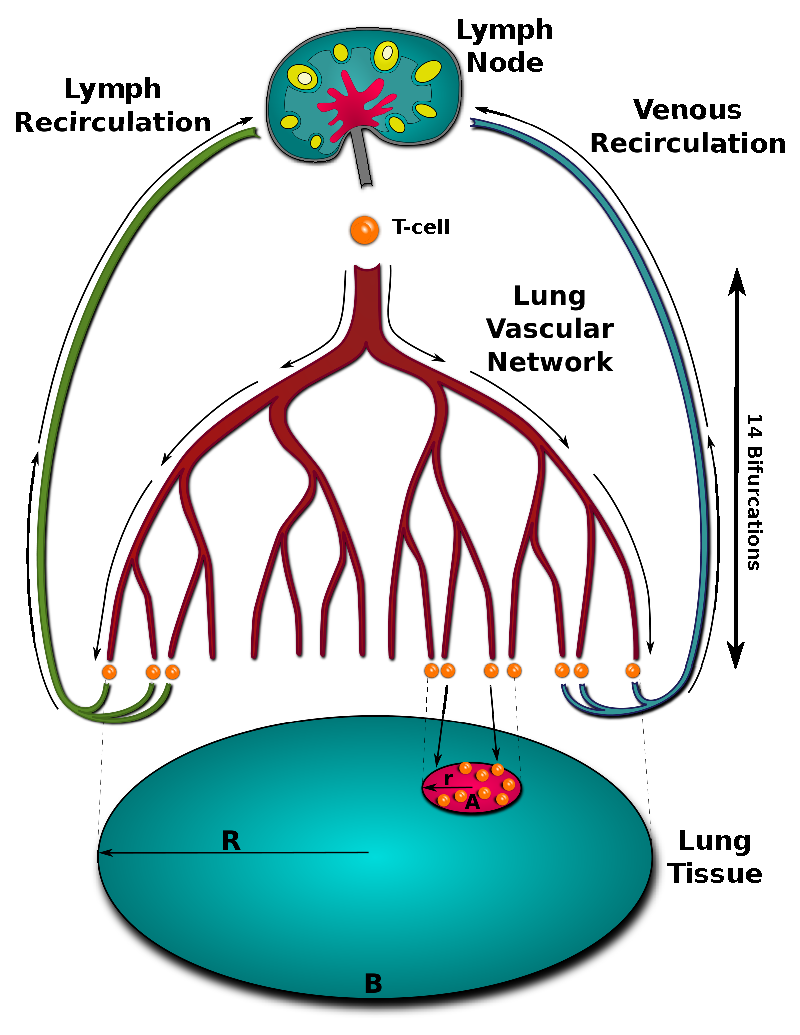
\includegraphics[width=4in]{Figure_1}
\end{center}
\caption{{\bf Model of T cell search.}  Activated T cells originate in the lymph node and enter the bloodstream after which they randomly navigate through 14 vascular bifurcations of the bronchial network.  Upon reaching a capillary, T cells exit into tissue if cytokine signal is present.  In the absence of signal, the T cell recirculates either through the lymph network or through the pulmonary vein back to the top of the network.}
\label{fig:systemchart}
\end{figure}

\begin{figure}[!ht]
\begin{center}
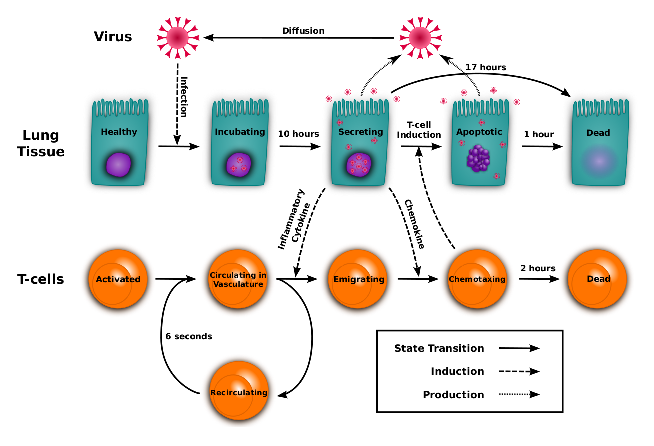
\includegraphics[width=4in]{Figure_2}
\end{center}
\caption{{\bf Visual representation of the model.}  Healthy epithelial cells infected by virus begin secreting virus after the incubation delay.  Activated T cells traverse the bronchial vascular network and may be recruited by inflammatory cytokine.  Chemotaxing T cells climb the chemokine gradient and induce apoptosis in infected cells.  Solid arrows represent a cell state transition from one behavior to another.  Dashed arrows display the mechanism used to induce a transition.  Dotted arrows indicate the production of new virus.}
\label{fig:modelchart}
\end{figure}

\begin{figure}[!ht]
\begin{center}
 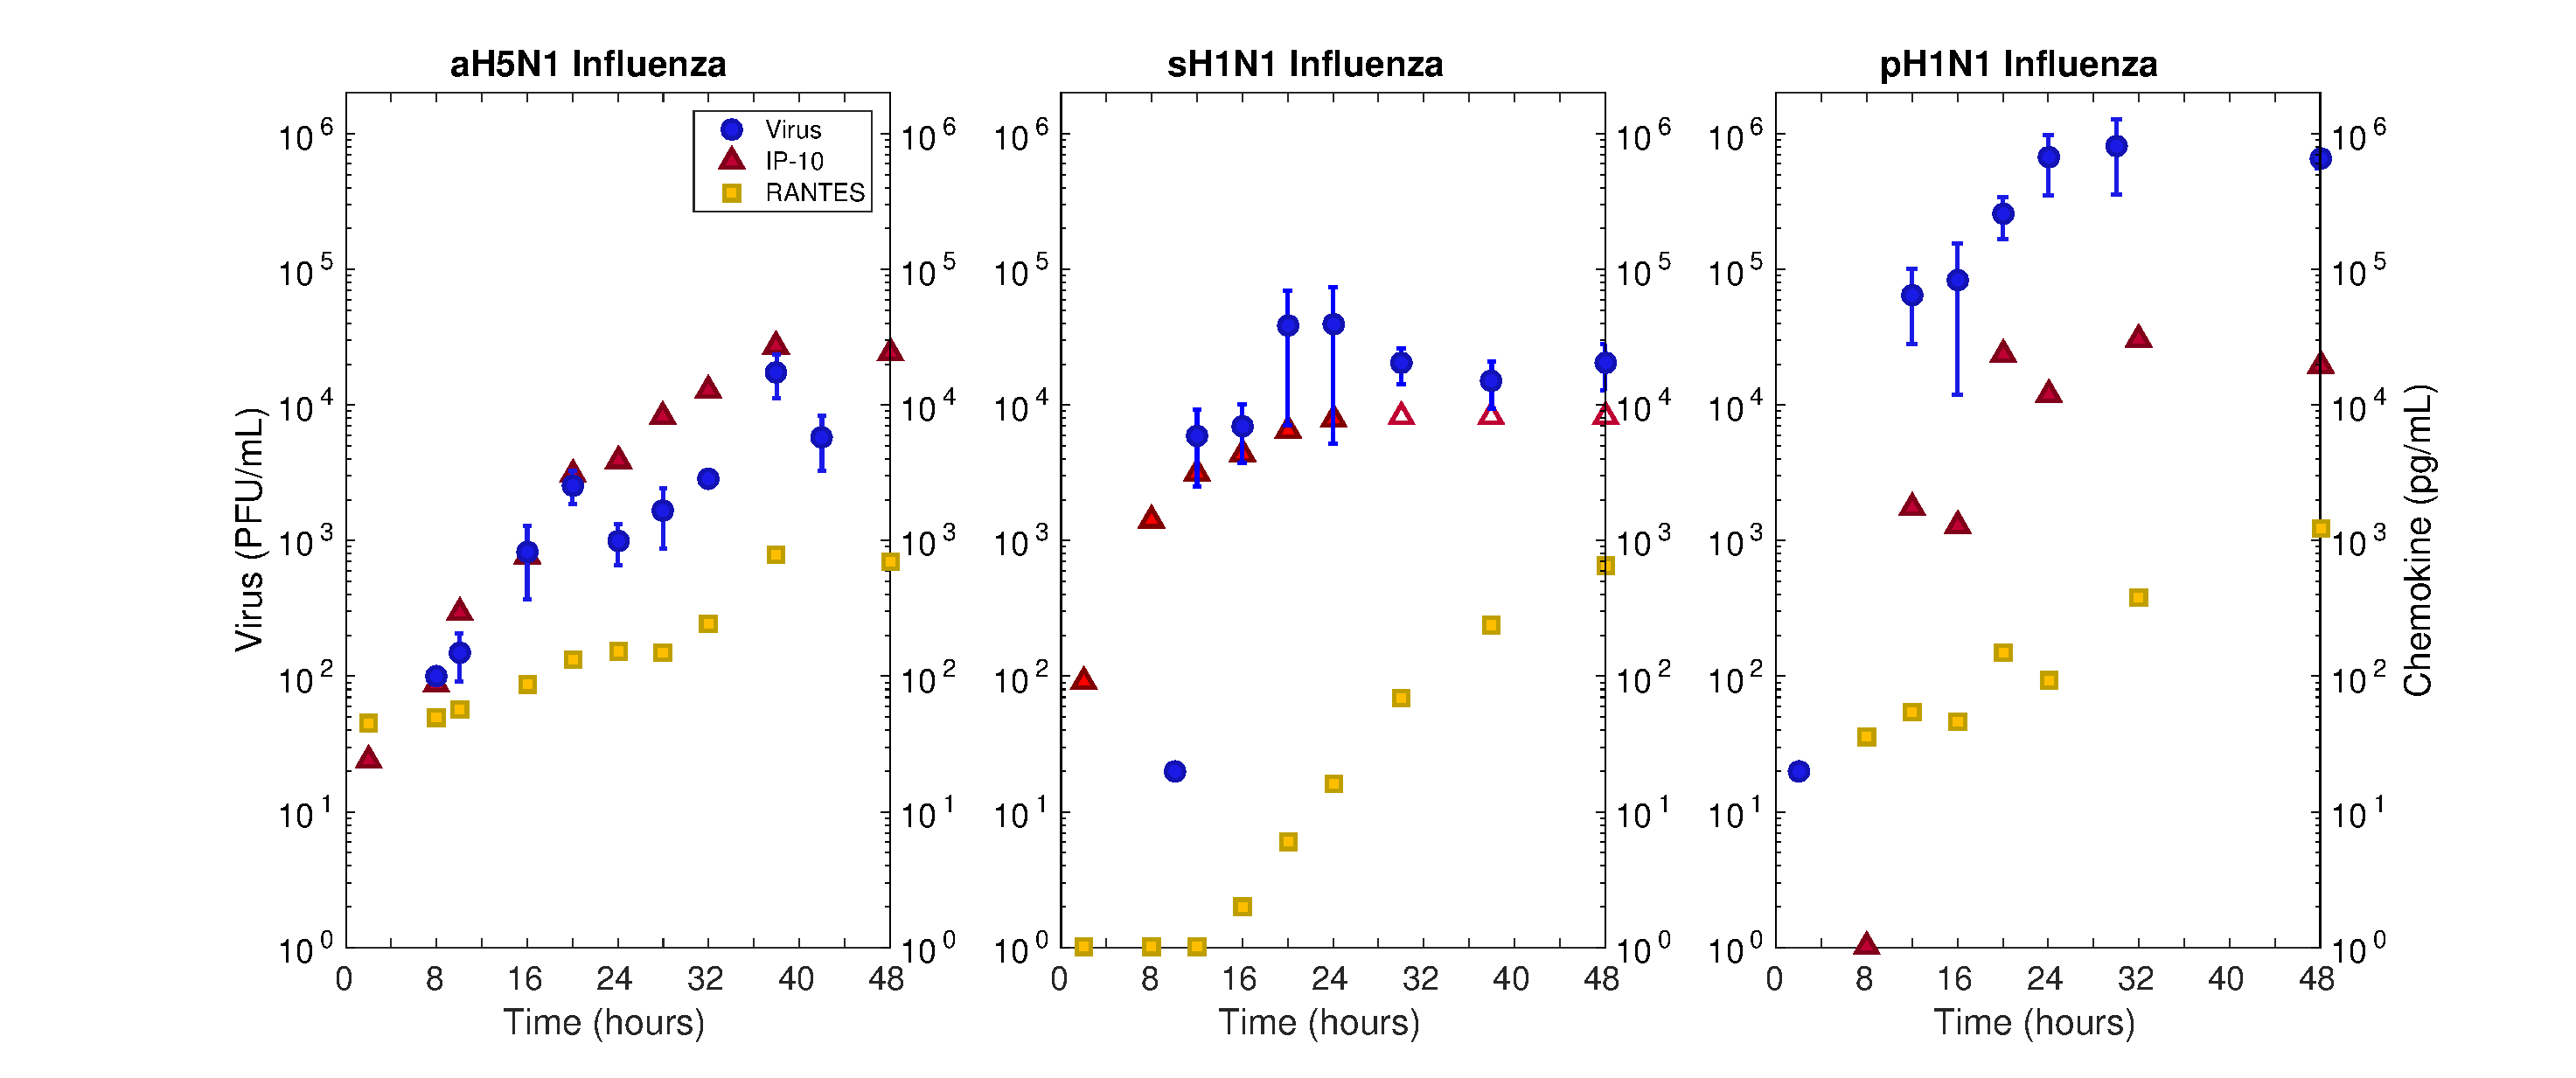
\includegraphics[width=\textwidth]{Figure_3}
 \end{center}
\caption{{\bf Empirical viral and cytokine titers for three strains of influenza: Avian H5N1, Seasonal sH1N1, and Pandemic pH1N1.}  Viral titer (blue circles) is in PFU/mL, and IP-10 (red triangle) and RANTES (green square) are shown in pg/mL.   sH1N1 IP-10 secretion exceeded measurement accuracy above 8500 pg/mL but these three values (empty red triangles) were not included in the model fitting.  An extended differential equation model from \cite{Mitchell2011} was fit to IP-10 and RANTES data (Section S2.1 Equation S1) .  These fits were used to obtain chemokine production values for use in the spatial CyCells model.  Human bronchial epithelial cells were infected at an MOI of 0.01 (10,000 virions) with one of the three strains of influenza.  Apical fluid for viral secretion and basal media for chemokine secretion was collected at the given time intervals post infection.  Viral culture was performed by a standard plaque assay and chemokine levels were measured using 30 $\mu$l aliots for a panel of 17 chemokines and cytokines (not shown).} 
 \label{fig:data}
\end{figure}

\begin{figure}[ht!]
\begin{center}
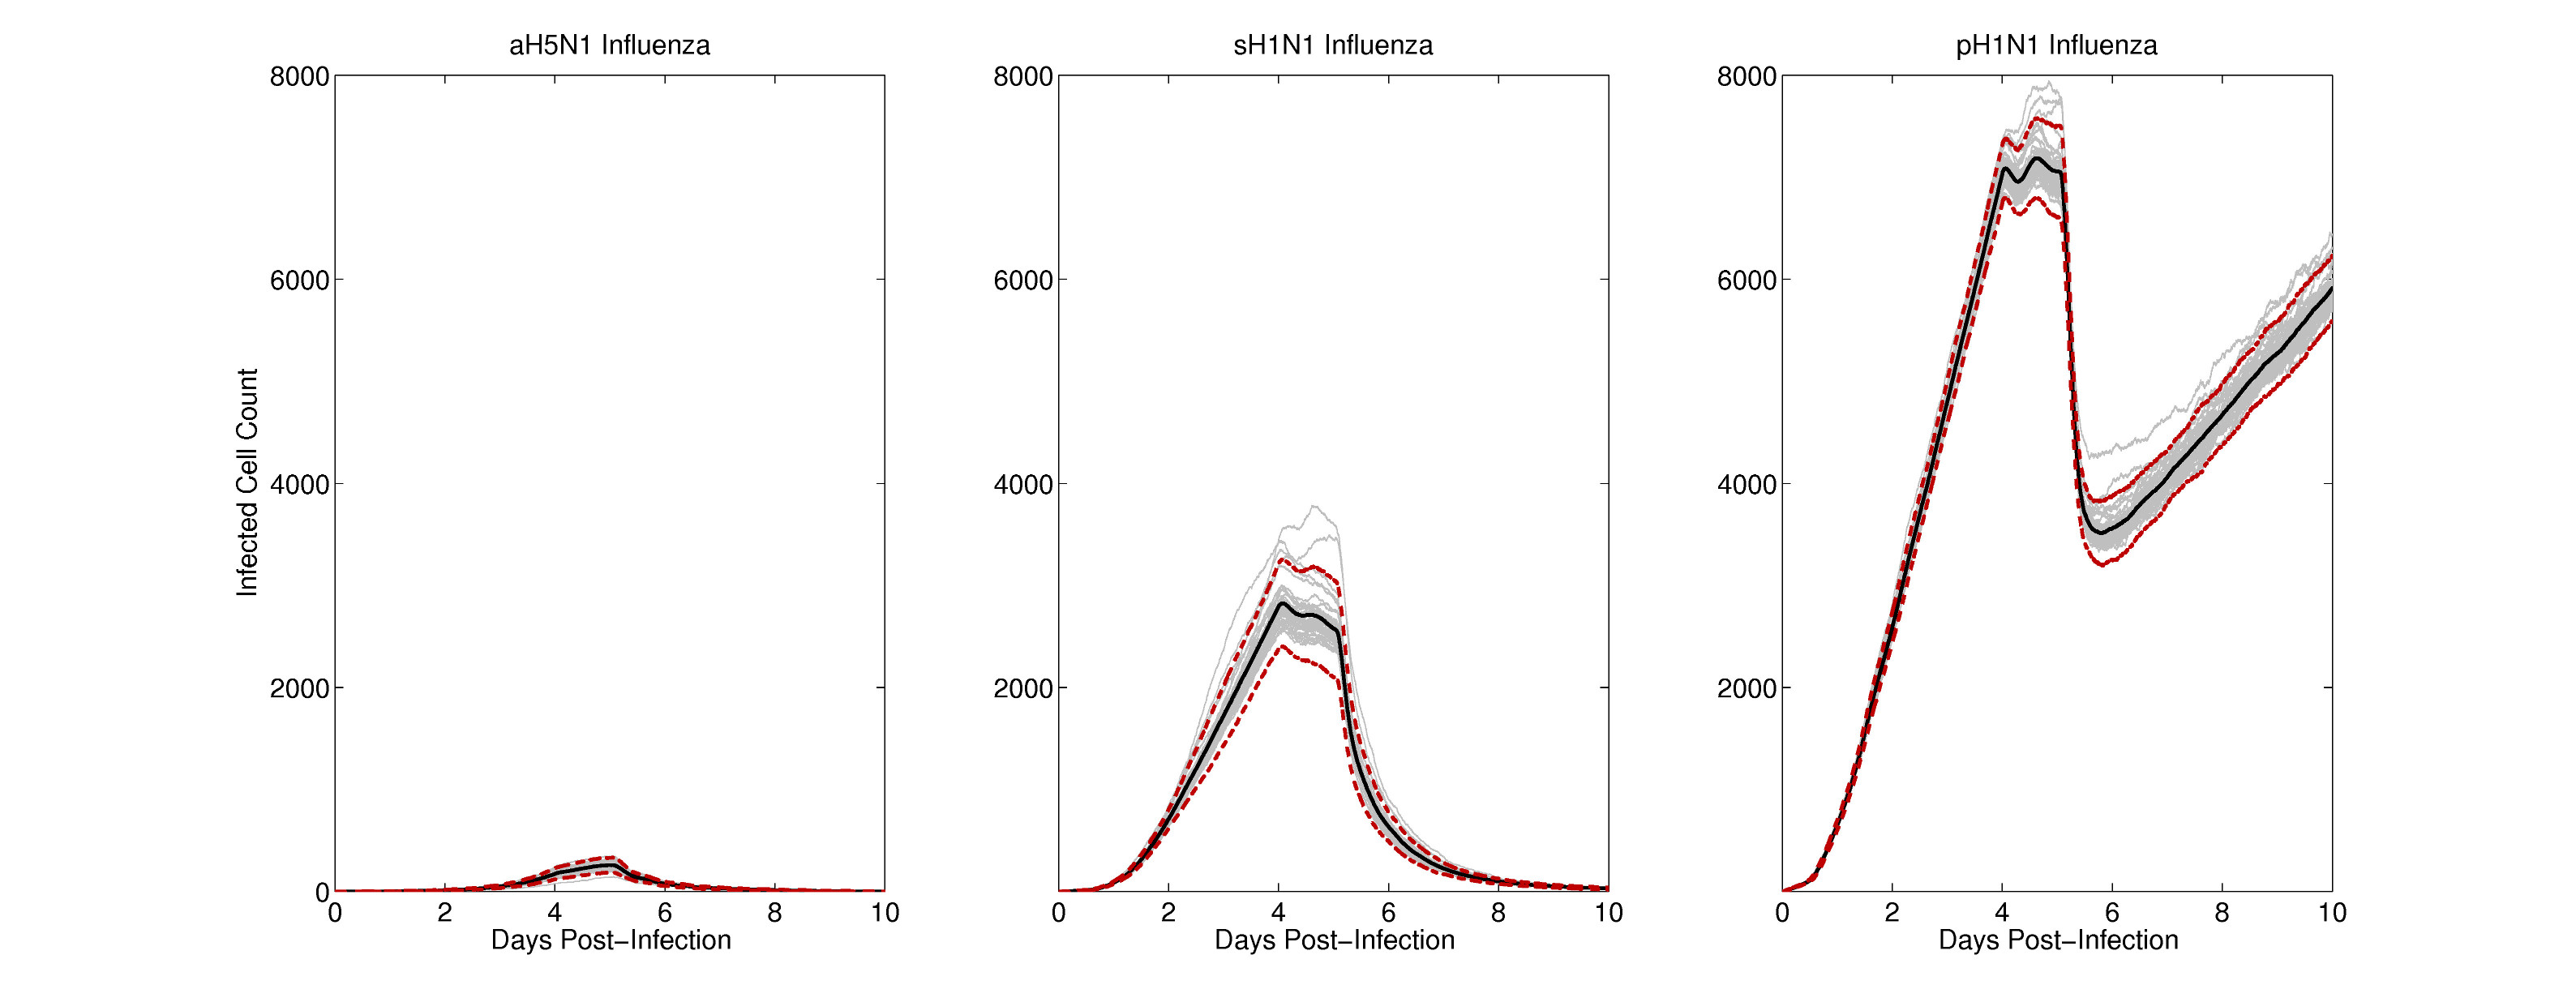
\includegraphics[width=\textwidth]{Figure_4}
 \end{center}
\caption{\textbf{Model results:} Time series plots of fifty runs of aH5N1 (A), sH1N1 (B), and pH1N1 (C) infections (gray). Each run took the calculated viral production and chemokine production rates for the three different strains of influenza as input (Table \ref{tab:strains}) and reported the total number of infected cells, including incubating, virus secreting and apoptotic, but not including dead cells.  Therefore the figures approximate the rate of plaque growth over time.  IP-10 and RANTES were simulated in each run, except for aH5N1, which  produced only RANTES.  Each run was initialized identically for each strain save for the random seed.  The middle line shows the mean while the red dashed lines show the 96\% credible confidence interval.} 
 \label{fig:variance}
\end{figure}

\begin{figure}[!ht]
\begin{center}
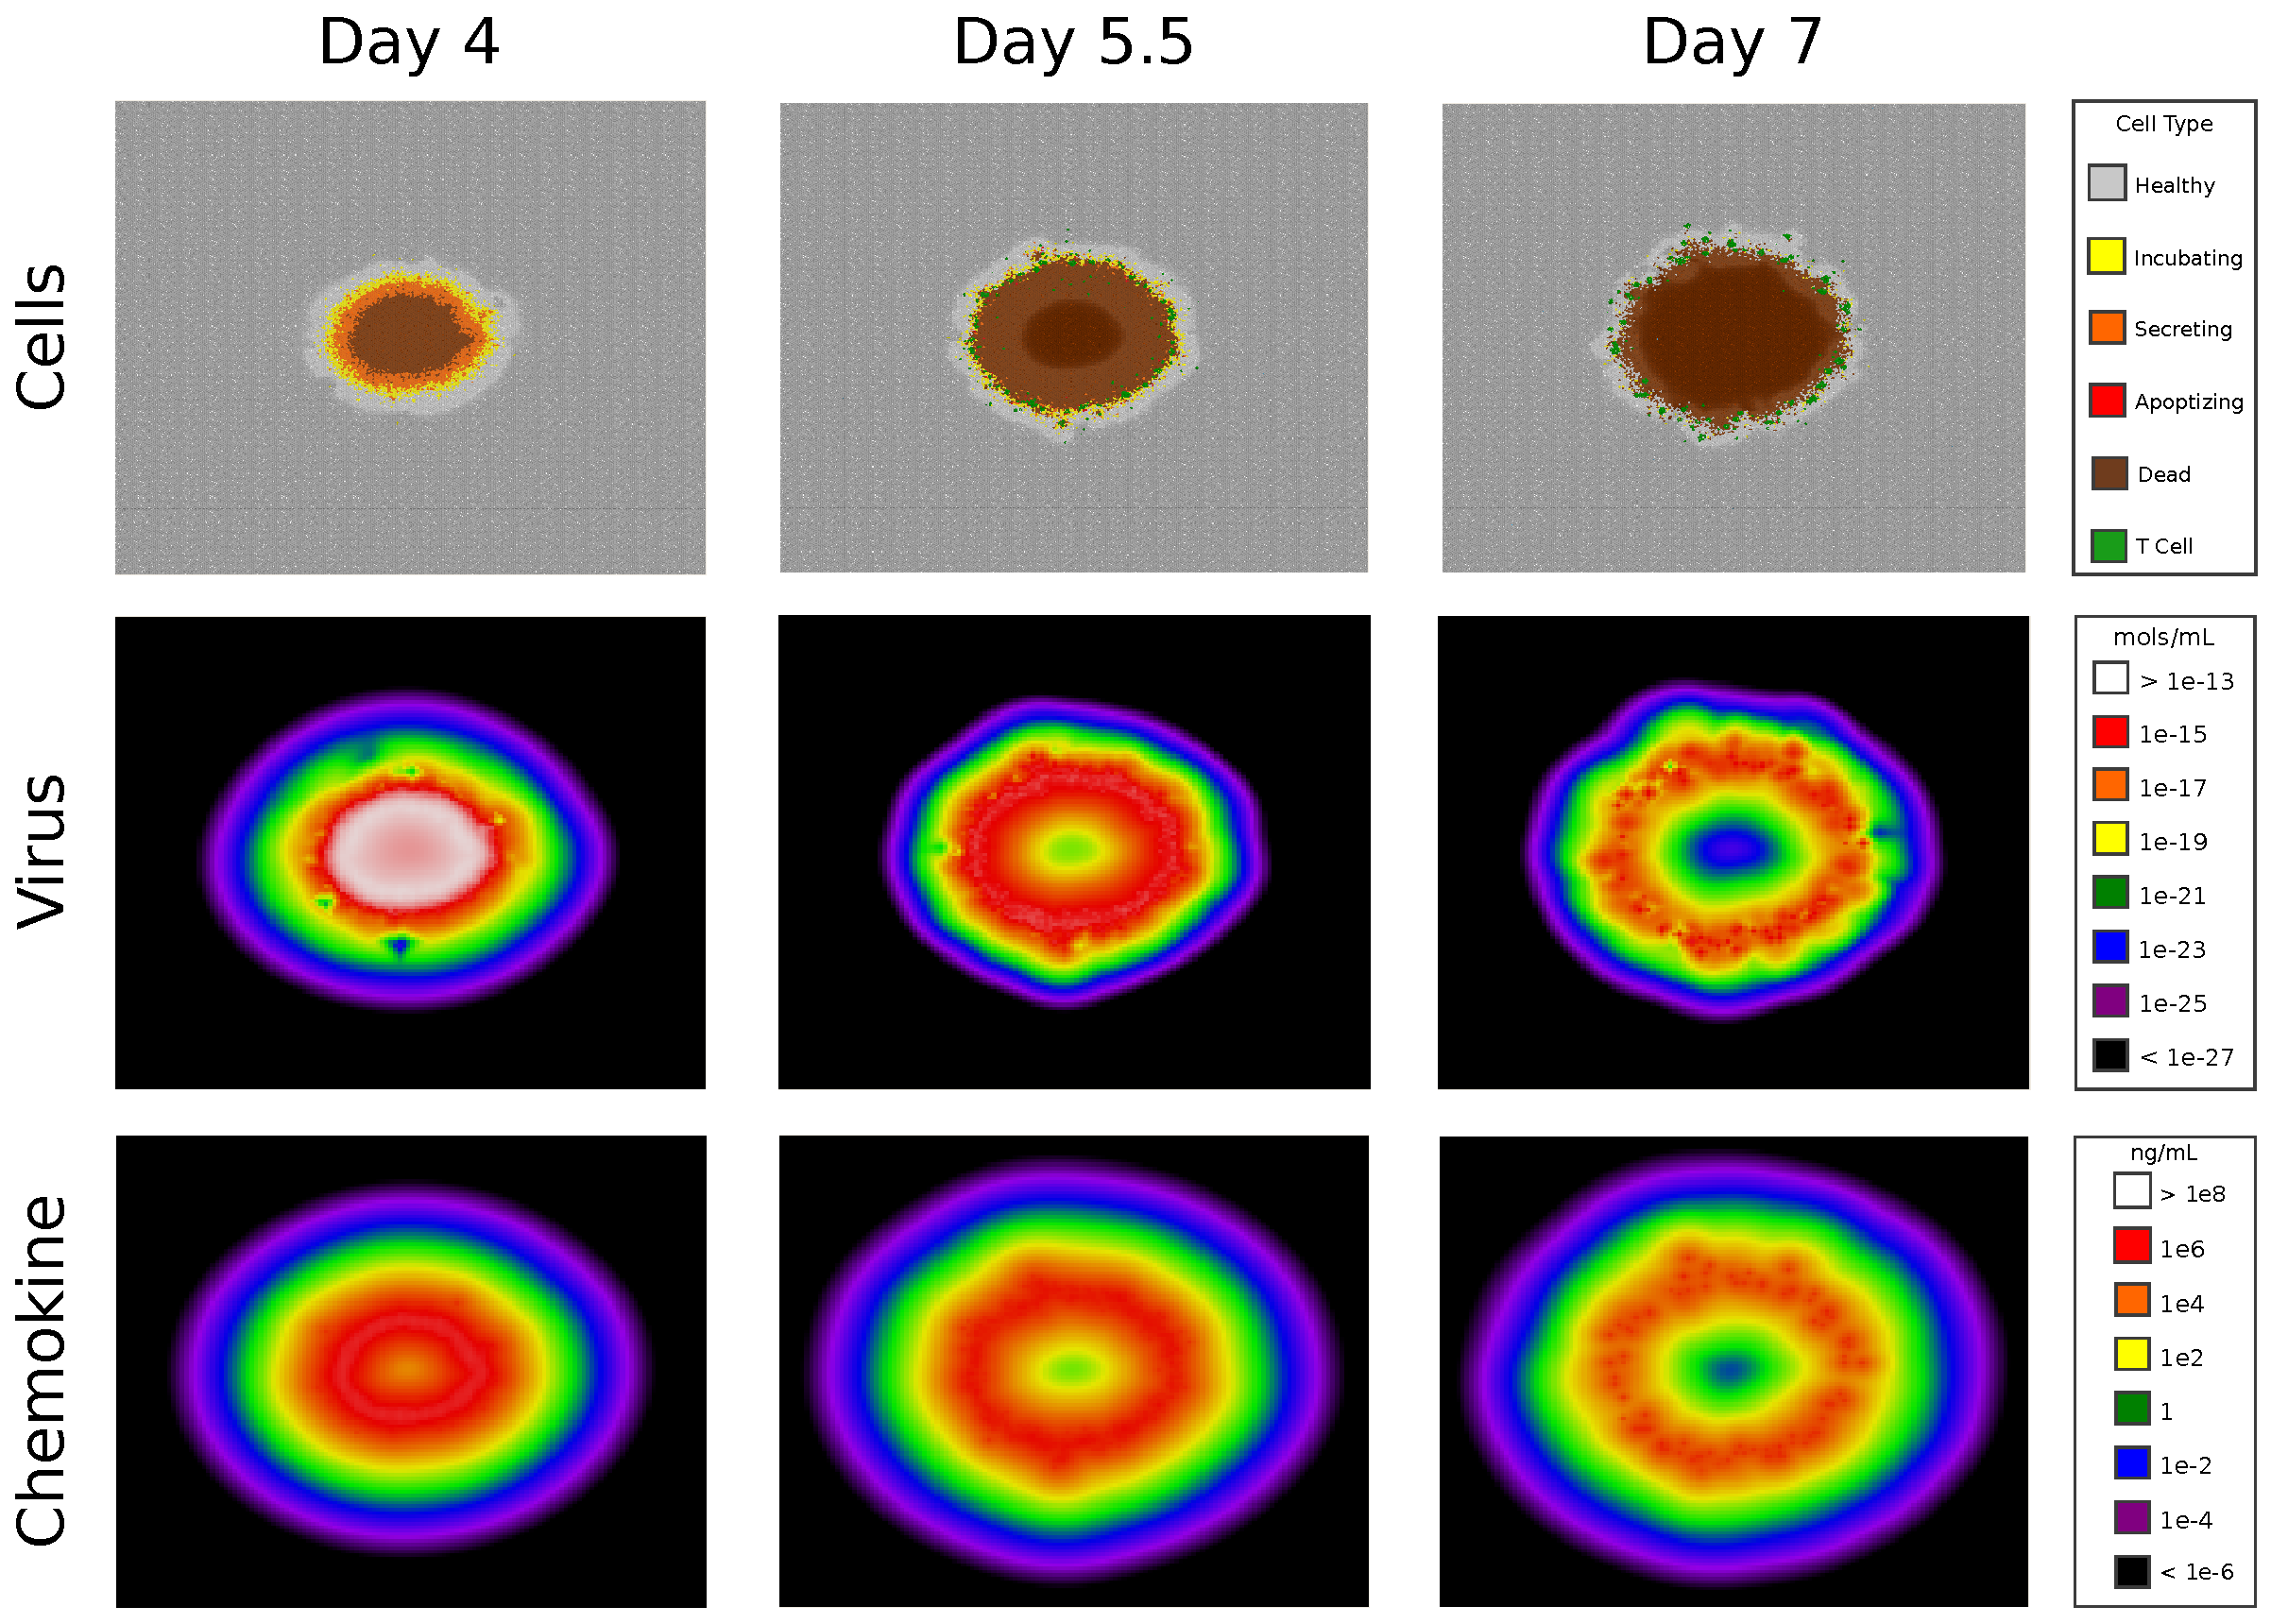
\includegraphics[width=\textwidth]{Figure_5}
 \end{center}
\caption{{\bf Simulated sH1N1 infection.} Screenshots from day 4, day 5.5, and day 7.  The top row shows the spreading focus of infection  through the color coding of individual cells:  healthy cells in uninfected tissue (gray),  virus-incubating cells (yellow), virus-secreting cells (orange), apoptotic cells (red), dead cells (brown), and T cells arriving at day 5 (green).  Free virus and chemokine particles are represented by compartmentalized concentrations of mols/mL and ng/mL.  Chemokine shown is an aggregate of total IP-10 and RANTES concentrations.  See Videos S1-S3 for an animated visualization of each row.} 
 \label{fig:cycells}
\end{figure}


\begin{figure}[!ht]
\begin{center}
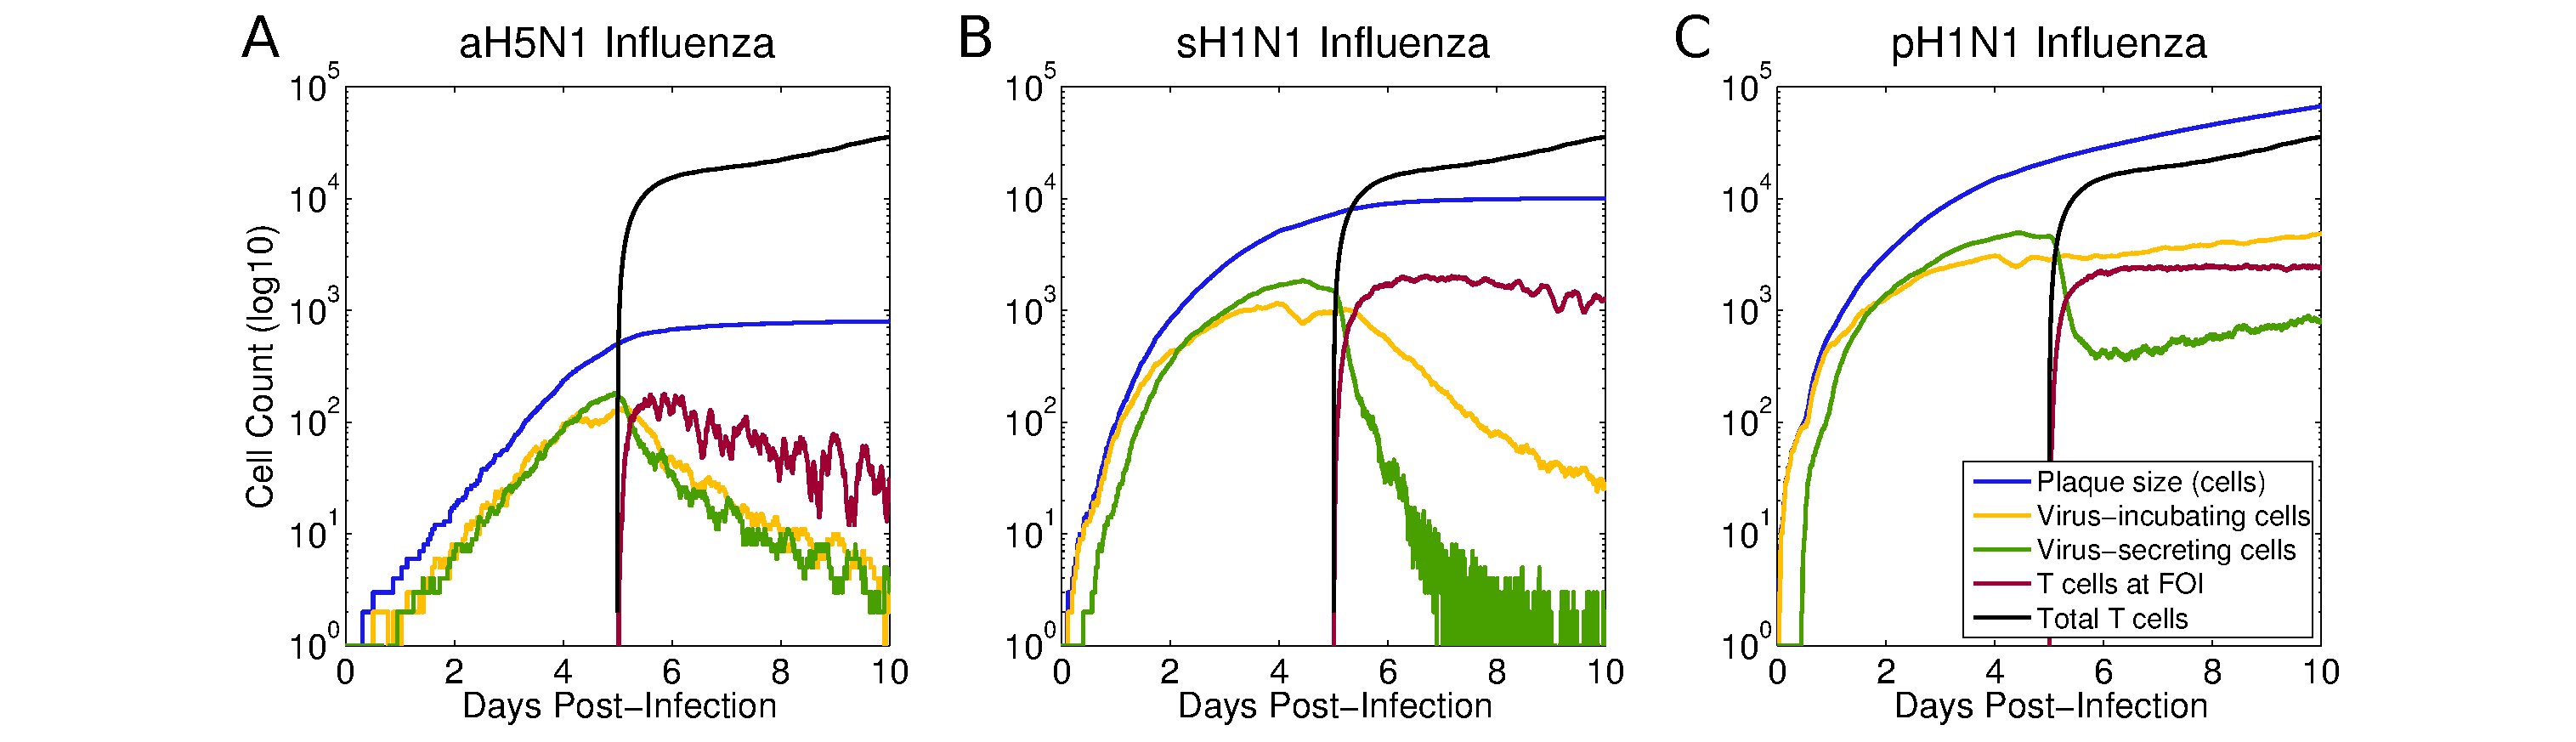
\includegraphics[width=\textwidth]{Figure_6}
 \end{center}
\caption{{\bf Simulated infections of aH5N1, sH1N1, and pH1N1.} Plotted values: total plaque size (blue), number of virus incubating cells (yellow), number of virus secreting cells (green), total number of T cells (black), and T cells at the focus of infection (FOI) (red).  T cells clear secreting and incubating cells in aH5N1, fail to clear incubating cells in sH1N1, and fail to clear either type of infected cell in pH1N1.  The number of incubating cells (yellow) after day 5 differs markedly among the three strains indicating that the T cells have differing success at controlling the infection.} 
 \label{fig:plaquesize}
\end{figure}


\begin{figure}[!ht]
\begin{center}
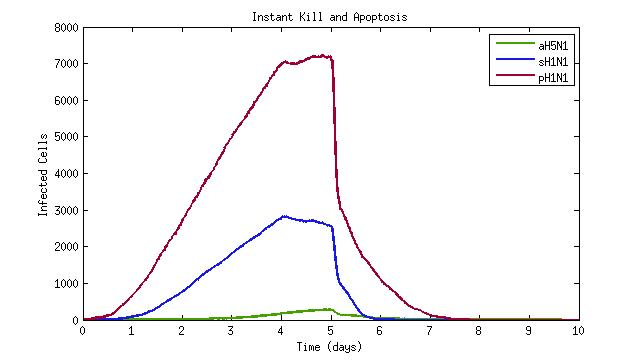
\includegraphics[width=4in]{Figure_7}
 \end{center}
\caption{{\bf Simulated infections of aH5N1, sH1N1, and pH1N1 with instant cell death.} The model results how that the combined delay of the T cell kill time and apoptosis time form a barrier to infection clearance.  Removing both delays results in infection clearance for all strains.}
 \label{fig:instantkill}
\end{figure}

\setcounter{figure}{0}
\renewcommand{\thefigure}{S\arabic{figure}}

\begin{figure}[ht!]
\begin{center}
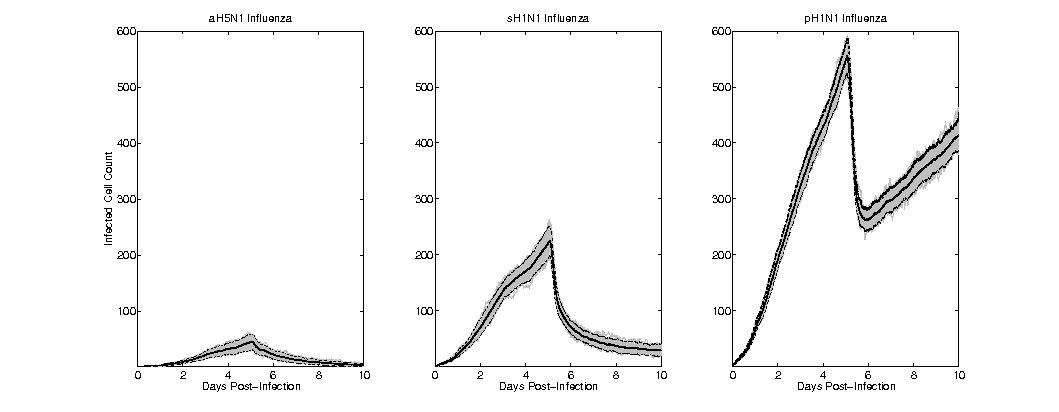
\includegraphics[width=\textwidth]{Figure_S1}
 \end{center}
\caption{{\bf Varying T cell sensitivity to chemokine.}  H5N1 model results use RANTES  only, and sH1N1 and pH1N1 use both IP-10 and RANTES. Total number of incubating, secreting and apoptotic cells are plotted for each infection.  The sensitivity value specifies the minimum level of chemokine concentration required for T cells to detect it.} 
\end{figure}


\begin{figure}[!ht]
\begin{center}
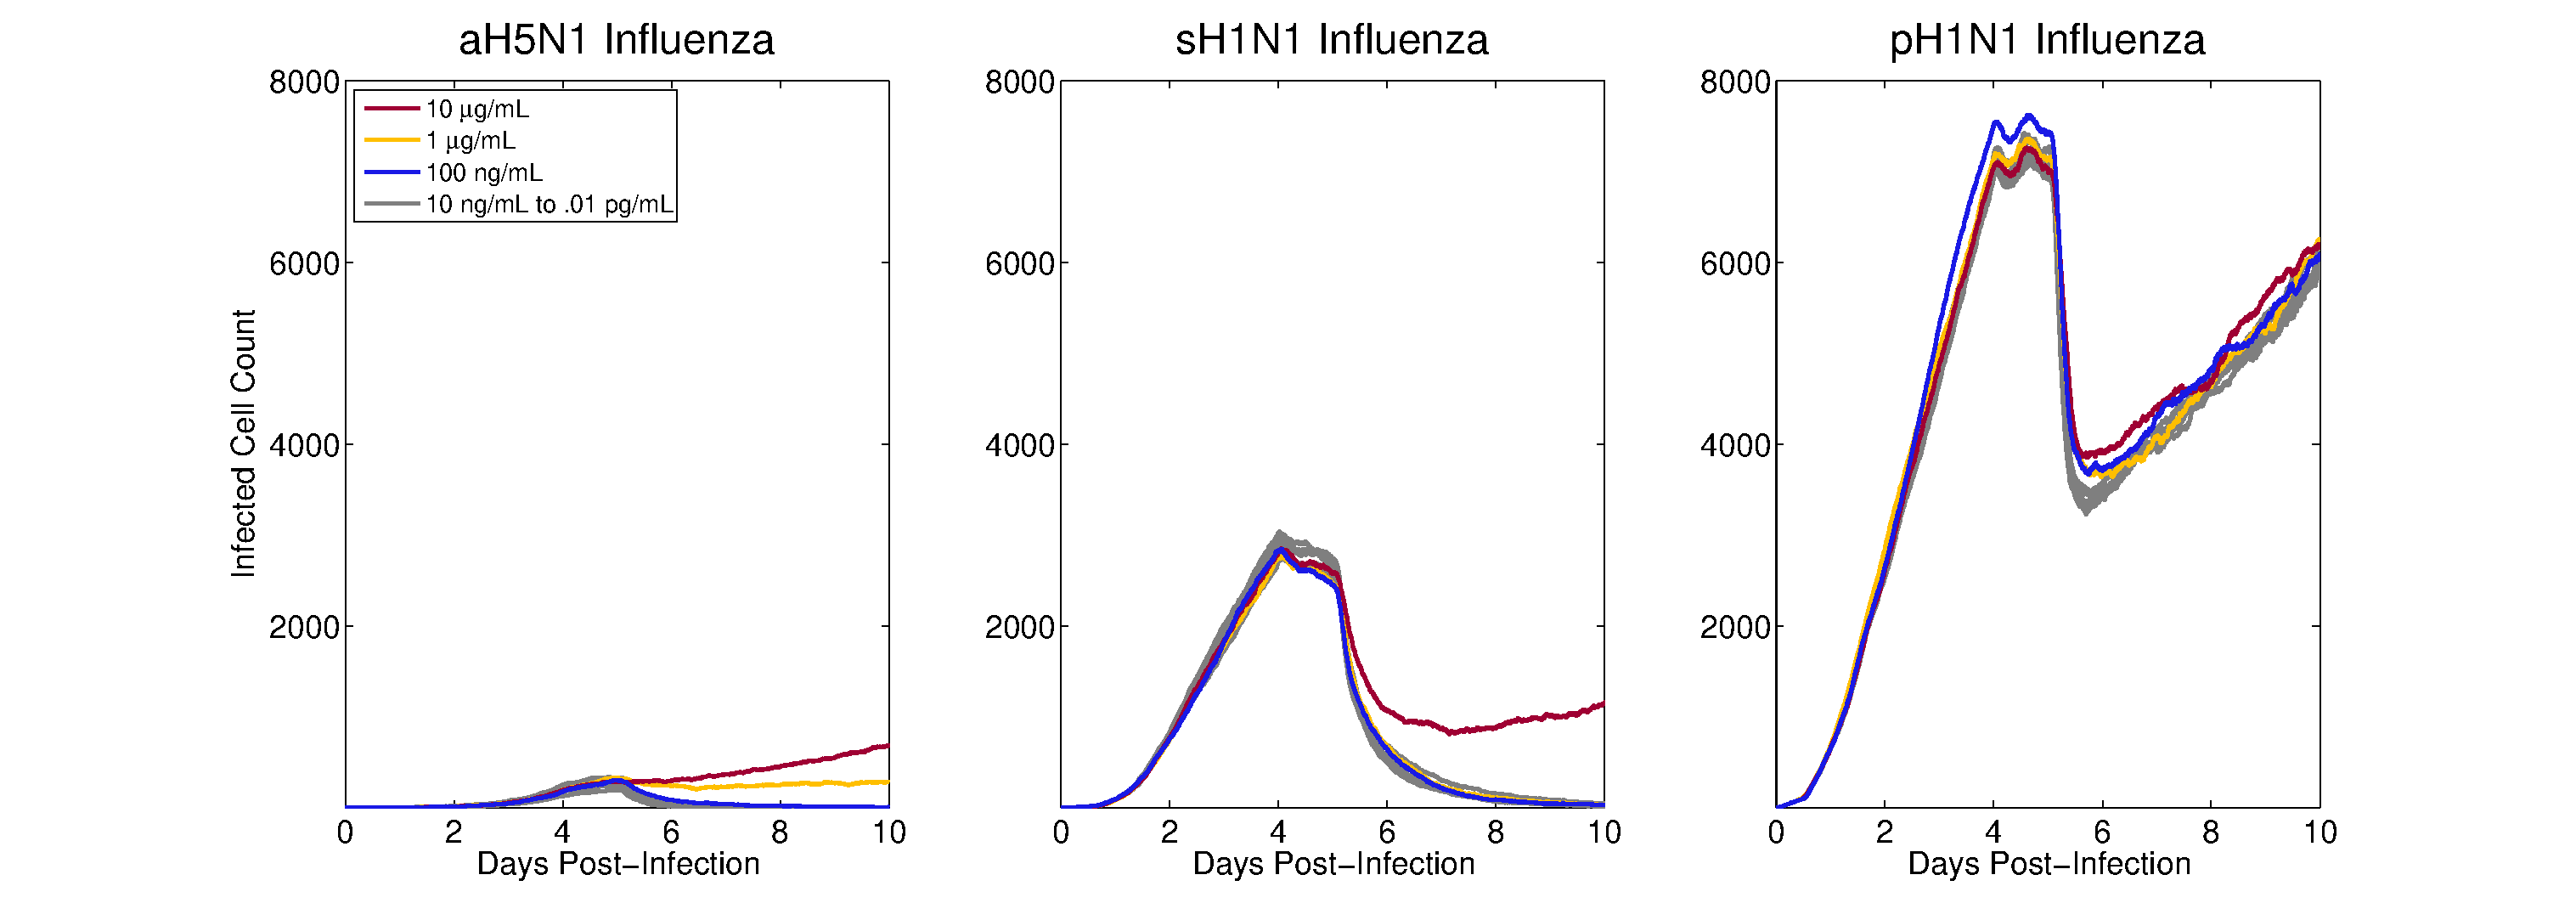
\includegraphics[width=4in]{Figure_S2}
 \end{center}
\caption{\textbf{Effects of different chemokine combinations.}  A) aH5N1 does not stimulate an IP-10 response.  B-C) sH1N1 and pH1N1 show no significant difference between IP-10 alone versus IP-10 and RANTES combined.} 
 \label{fig:sensitivity}
\end{figure}

\setcounter{figure}{0}
\renewcommand{\figurename}{Video}

\begin{figure}[ht!]
\caption{The first of three overlaid videos of a representative seasonal H1N1 infection.  This video spans the 10 day infection and shows the cells as they transition from healthy to infected to dead.  T cells show half way through the simulation.  Healthy cells are gray, virus-incubating cells are yellow, virus-secreting cells are orange, apoptotic cells are red, and T cells are green.} 
 \label{video:cell_view}
\end{figure}

\begin{figure}[ht!]
\caption{The second of three overlaid videos of a representative seasonal H1N1 infection.  This video spans the 10 day infection and shows the virus concentration.  Notice the volatility when T cells arrive halfway through the simulation.  Virus concentration ranges from 1e-13 mols/mL (white) to 1e-27 mols/mL (black).  Refer to Figure 5 for the detailed legend. } 
 \label{video:virus_view}
\end{figure}

\begin{figure}[ht!]
\caption{The third of three overlaid videos of a representative seasonal H1N1 infection.  This video spans the 10 day infection and shows the chemokine concentration.  Notice the volatility when T cells arrive halfway through the simulation.  Chemokine concentration ranges from 1e8 ng/mL (white) to 1e-6 ng/mL (black).  Refer to Figure 5 for the detailed legend. } 
 \label{video:chemokine_view}
\end{figure}

\begin{figure}[ht!]
\caption{A closer look at the 2009 pandemic simulation.  This video shows the infection from day 6 to day 7 with each frame spanning 60 simulated seconds.  Healthy cells are gray, virus-incubating cells are yellow, virus-secreting cells are orange, apoptotic cells are red, and T cells are green.  Note the high proportion of virus-secreting cells (orange) early on.  As time passes, secreting cells are gradually contained to the point where they become very sparse.  T cell clumping often prevents the T cells from quick discovery of new secreting cells.}
\end{figure}

\pagebreak

\section*{Tables}
%\begin{table}[!ht]
%\caption{
%\bf{Table title}}
%\begin{tabular}{|c|c|c|}
%table information
%\end{tabular}
%\begin{flushleft}Table caption
%\end{flushleft}
%\label{tab:label}
% \end{table}



\begin{table}[!ht]
\centering
\begin{tabular}{ | r | c | c | c | }
  \hline                        
  \multicolumn{1}{|c|}{\multirow{2}{*}{Strain}} & IP-10 Production & RANTES Production & Viral Production \\
   & \footnotesize{$(pg/s\cdot cell)$}  & \footnotesize{$(pg/s\cdot cell)$} &  \footnotesize{$(PFU/s\cdot cell)$} \\
  \hline
  \multirow{2}{*}{Avian H5N1} & 2.0e-4 &  1.3e-5 & 5.4e-5 \\
   &  \footnotesize{8.4e-5 --- 4.2e-4} & \footnotesize{7.9e-6 --- 1.9e-5} & \footnotesize{4.4e-5 --- 3.7e-4}\\ 
   \hline
  \multirow{2}{*}{Seasonal H1N1} & 1.8e-4 &  8.9e-7 & 3.8e-4 \\
   & \footnotesize{1.2e-4 --- 3.0e-4} & \footnotesize{4.8e-7 --- 1.6e-6} & \footnotesize{2.8e-4 --- 1.5e-3}\\
   \hline
  \multirow{2}{*}{Pandemic H1N1} & 8.7e-5 &  4.3e-6 & 5.1e-3 \\
   & \footnotesize{1.7e-5 --- 7.1e-4} & \footnotesize{5.0e-7 --- 3.5e-5} & \footnotesize{2.8e-3 --- 5.3e-3} \\
  \hline
\end{tabular}
\caption{Strain-specific parameters.  Small text values show 95\% confidence intervals resulting from 1,000 bootstrapping runs for each parameter \cite{Wu1986}.  Bootstrapping for the chemokine values was performed using the original fit of Eq. S1 to the data in Fig.~\ref{fig:data} to produce new data sets.  Viral production values and confidence intervals are taken from \cite{Mitchell2011}.}
\label{tab:strains}
\end{table}

\begin{table}[!ht]
\begin{center}
\begin{tabular}{| l | c | l l l | c |}
  \hline                        
  Referenced Parameters & Units & Min & Value & Max & Source \\
  \hline
  $^{\dagger}$Viral Diffusion in Airway & \textit{$\mu$m$^2$/s} & 3.18e-4 & \textbf{3.18e-2} & 3.18  & \cite{Beauchemin2006} \\
  $^{\dagger}$Viral Decay in Airway & \textit{day$^{-1}$} & 0.01 & \textbf{1} & 100 & \cite{Lee2009} \\
  Chemokine Diffusion Rate & \textit{$\mu$m$^2$/s} & 3.18e-3 & \textbf{.318} & 318 & \cite{Beauchemin2006} \\
  Incubation Time & \textit{hours} & 5 & \textbf{10} & 20 & \cite{Mitchell2011} \\
  Epithelial Cell Radius & \textit{$\mu$m} & | & \textbf{5} & | & \cite{Elbert1999} \\
  T Cell Radius & \textit{$\mu$m} & | & \textbf{5} & | & \cite{abbas2011cellular} \\
  T Cell Production Rate & \textit{cells/h} & 125 & \textbf{1,257} & 3,750 & \cite{Miao2010} \\ 
  T Cell Speed & \textit{$\mu$m/min} & 6e-2 & \textbf{6} & 600 & \cite{Egen2011} \\
  Blood Circulation Time & \textit{seconds} & 1 & \textbf{6} & 3,600 & \cite{Banerjee2010b} \\
  T Cell Sensitivity to Chemokine & \textit{ng/mL} & | & \textbf{100} & | & \cite{Nandagopal2011} \\
  Onset of T Cell Lymph Node Exit & \textit{days }& | & \textbf{5} & | & \cite{Banerjee2011} \\
  $^{\dagger}$IgM Viral Decay Factor & | & 1 & \textbf{10} & 1,000 & \cite{Diamond2003} \\
  IgM Onset & \textit{days} & | & \textbf{4} & | & \cite{Diamond2003} \\
  \hline
  \hline                        
  Estimated Parameters & Units & Min & Value & Max & Footnote \\
  \hline
  Chemokine Decay Rate & \textit{Hz} & 3.8e-6 & \textbf{3.8e-4} & 3.8e-2 & 1\\
  $^{\dagger}$Infectivity & \textit{min/virion} & 12 & \textbf{120} & 1,200   &  2 \\
  Expression Time & \textit{min} & 100 & \textbf{1,000} & 3,000 & \cite{Mitchell2011}$^3$ \\
  T Cell Expected Kill Time & \textit{min} & 0 & \textbf{10} & 100 & 4 \\
  Apoptosis Time & \textit{hours} & 0 & \textbf{1} & 2 & \cite{Ganusov2008}$^5$ \\
  T Cell Age (at FOI) & \textit{min} & 12 & \textbf{120} & 1,200 & 6 \\
  T Cell Age (in Blood) & \textit{days} & 0.04 & \textbf{4} & 400 & 6 \\
  \hline  
\end{tabular}
\caption{Default values used for the model in bold.  Min and max represent the extreme values tested in the sensitivity analysis (Table~\ref{tab:sensitivity} and Fig.~S3-5).  $^{\dagger}$ denotes parameters determined to be sensitive by the sensitivity analysis.  Values were taken from experimental literature if possible and from earlier modeling papers if not.  Parameters not found in literature were estimated as follows.  1) Corresponds to a 30 minute half-life.  2) Epithelial cells are infected at a probabilistic rate such that the expected time for infection in the presence of a single virion is 2 hours.  This scales linearly with the number of virions in the cell's vicinity.  3) Chosen as a plausible median time (1,000 minutes) between 6 hours and 24 hours.  4) T cells induce apoptosis in nearby virus-secreting epithelial cells at a probabilistic rate such that the expected time to induce apoptosis is 10 minutes.  This rate does not scale with T cell numbers.  5) Calculated for low T cell densities.  6) Chosen to be at the lower end of biologically plausible values because increased T cell counts are shown not to affect the model behavior. }
\label{tab:parameters}
\end{center}
\end{table}
% 7) IgM presence is abstracted by increasing viral decay by a factor of ten. $^\ddagger$Activated T Cell.  $^\ast$Focus of Infection.


\begin{table}[!ht]
\begin{center}
\begin{tabular}{| c | l | c c c |}
  \hline                        
  Category & Parameter & Avian H5N1 & Seasonal H1N1 & Pandemic H1N1 \\
  \hline
  \multirow{3}{*}{Chemokine} & Chemokine Decay Rate & \cellcolor{blue!30}bounded stable & \cellcolor{blue!30}bounded stable & \cellcolor{green!50}stable \\
  & Chemokine Diffusion Rate & \cellcolor{blue!30}bounded stable & \cellcolor{green!50}stable& \cellcolor{green!50}stable \\
  & Chemokine Secretion Rate & \cellcolor{blue!30}bounded stable & \cellcolor{green!50}stable & \cellcolor{green!50}stable \\
  \hline
  \multirow{6}{*}{T Cell} & Circulation Time & \cellcolor{blue!30}bounded stable & \cellcolor{blue!30}bounded stable & \cellcolor{blue!30}bounded stable \\
  & T Cell Kill Rate & \cellcolor{green!50}stable & \cellcolor{blue!30}bounded stable & \cellcolor{blue!30}bounded stable \\
  & T Cell Velocity & \cellcolor{green!50}stable & \cellcolor{blue!30}bounded stable & \cellcolor{blue!30}bounded stable \\
  & Circulating Decay Rate & \cellcolor{green!50}stable & \cellcolor{blue!30}bounded stable& \cellcolor{blue!30}bounded stable \\
  & Found Decay Rate & \cellcolor{green!50}stable & \cellcolor{blue!30}bounded stable & \cellcolor{blue!30}bounded stable \\
  & T Cell Production Rate & \cellcolor{blue!30}bounded stable & \cellcolor{blue!30}bounded stable & \cellcolor{blue!30}bounded stable \\
  \hline
  \multirow{3}{*}{Delay} & Apoptosis Time & \cellcolor{green!50}stable & \cellcolor{green!50}stable & \cellcolor{green!50}stable \\
  & Expression Time & \cellcolor{yellow!50}peak change & \cellcolor{yellow!50}peak change & \cellcolor{yellow!50}peak change \\
  & Incubation Time &  \cellcolor{yellow!50}peak change & \cellcolor{yellow!50}peak change & \cellcolor{yellow!50}peak change \\
  \hline 
  \multirow{4}{*}{Virus} & Viral Response to IgM & \cellcolor{red!40}sensitive & \cellcolor{red!40}sensitive & \cellcolor{red!40}sensitive \\
  & Infectivity & \cellcolor{red!40}sensitive & \cellcolor{red!40}sensitive & \cellcolor{red!40}sensitive \\
  & Viral Decay Rate & \cellcolor{red!40}sensitive & \cellcolor{red!40}sensitive & \cellcolor{red!40}sensitive \\
  & Viral Diffusion Rate & \cellcolor{red!40}sensitive & \cellcolor{red!40}sensitive & \cellcolor{red!40}sensitive \\
  \hline  
\end{tabular}
\caption{\textbf{Sensitivity Results:} The above parameters were varied over predetermined ranges in isolation, resulting in new model runs for every new value tested.  The results of the sensitivity analysis were then qualitatively evaluated for each individual parameter.  A model run's behavior was determined by examining the height of the peak of the infection at day 5 post-infection and the number of infected cells at day 10 post-infection.  Each combination of influenza strain and free parameter was classified as belonging to one of four categories.  Parameters were classified as \textbf{stable} if all runs follow the same behavior, \textbf{bounded stable} if intermediate parameter adjustments did not affect the model's behavior, even if the more extreme adjustments did, \textbf{peak change} if the peak of the infection differs but the result at day 10 is the same, and \textbf{sensitive} if any level of change in the parameter affects the resulting model behavior.}
\label{tab:sensitivity}
\end{center}
\end{table}
% 7) IgM presence is abstracted by increasing viral decay by a factor of ten. $^\ddagger$Activated T Cell.  $^\ast$Focus of Infection.



\end{document}

